\documentclass{article}

\usepackage{amsmath, amsfonts, amssymb}
\usepackage{amsthm}
\usepackage{hyperref}
\usepackage{tikz-cd}
\usepackage{graphicx}
\usepackage{enumitem}
\usepackage[english]{babel}

\graphicspath{{graphics/}}

\author{Matthew Dupraz}
\title{Elliptic Curves over $\mathbb{C}$ and over Finite Fields}

\newtheorem{theorem}{Theorem}[section]
\newtheorem{corollary}{Corollary}[theorem]
\newtheorem{lemma}[theorem]{Lemma}
\newtheorem{proposition}[theorem]{Proposition}

\theoremstyle{definition}
\newtheorem{definition}{Definition}[section]
\newtheorem*{notation}{Notation}

\theoremstyle{remark}
\newtheorem*{remark}{Remark}

\newcommand{\cl}{\overline}
\newcommand{\proj}{\mathbb{P}}
\newcommand{\A}{\mathbb{A}}
\newcommand{\F}{\mathbb{F}}
\newcommand{\C}{\mathbb{C}}
\newcommand{\R}{\mathbb{R}}
\newcommand{\Q}{\mathbb{Q}}
\newcommand{\N}{\mathbb{N}}
\newcommand{\Z}{\mathbb{Z}}
\newcommand{\T}{\mathbb{T}}
\renewcommand{\O}{\mathcal{O}}
\newcommand{\chr}{\operatorname{char}}
\newcommand{\Frac}{\operatorname{Frac}}
\renewcommand{\div}{\operatorname{div}}
\newcommand{\im}{\operatorname{im}}
\newcommand{\id}{\operatorname{id}}
\newcommand{\rk}{\operatorname{rk}}
\newcommand{\tr}{\operatorname{tr}}
\newcommand{\res}{\operatorname{res}}
\newcommand{\ord}{\operatorname{ord}}
\newcommand{\End}{\operatorname{End}}
\newcommand{\Hom}{\operatorname{Hom}}
\newcommand{\ts}{\textsuperscript}

\begin{document}

\maketitle
\section{Algebraic Varieties}

\comment{Motivate the definitions,
remind important definitions from the course}

\begin{definition}
	Let $V$ be a algebraic variety. Let $L$ be a subfield of $K$.
	We say that $V$ is \emph{defined over} $L$ when the ideal of
	$V$ can be generated by polynomials in $L[X]$.
	We will denote this by $V/L$.
\end{definition}

\begin{definition}
	Let $L \subseteq K$ a subfield.
	We define the set $\A^n(L) \subseteq \A^n$ as
	\begin{equation*}
		\A^n(L) := \{(x_1, \dots, x_n) \in \A^n \mid x_i \in L\}.
	\end{equation*}
	We call this set the \emph{set of $L$-rational} points of $\A^n$.
	Similarly, we define
	\begin{equation*}
		\proj^n(L) := \{[x_1, \dots, x_{n+1}) \in \proj^n \mid x_i \in L\},
	\end{equation*}
	the set of $L$-rational points of $\proj^n$.
\end{definition}

\begin{definition}
	Let $L \subset K$ a subfield.
	Let $V/L$ be an algebraic variety defined over $L$.
 	We define the set
	of $L$-rational points of $V$
	\begin{equation*}
		V(L) := 
		\begin{cases}
			V\cap\A^n(L) &\textrm{if $V$ is affine;}\\
			V\cap\proj^n(L) &\textrm{if $V$ is projective.}
		\end{cases}
	\end{equation*}
\end{definition}

The projective space $\proj^n$ can be covered by copies of $\A^n$. Define
\begin{equation*}
	U_i := \{[x_0, \dots, x_n] \in \proj^n \mid x_i \neq 0\},
\end{equation*}
then $U_i$ is isomorphic to $\A^n$ via the chart
\begin{equation*}
	\phi_i: U_i \to \A^n, [x_0, \dots, x_n] \mapsto \left(\frac{x_1}{x_i}, \dots,
		\frac{x_{i-1}}{x_i}, \frac{x_{i+1}}{x_i}, \dots, 
		\frac{x_n}{x_i}\right)
\end{equation*}

\begin{notation}
	Thanks to the above isomorphism, we can see $\A^n$ as a chosen
	$U_i \subset \proj^n$. Hence we can see any affine variety
	$V \subseteq \A^n$ as a subset of $\proj^n$. Similarly, if $V \subseteq
	\proj^n$ is a projective variety,
	then for a chosen $\A^n \subseteq \proj^n$,
	$V \cap \A^n$ is an affine variety.
\end{notation}
\comment{Not sure I want to keep this notation}

\begin{definition}
	For $V \subseteq \proj^n$ a subset, we define $\cl{V}$ the (Zariski)
	\emph{closure}, the closure of $V$ in the Zariski topology of $\proj^n$.
\end{definition}

\begin{proposition}
	\begin{enumerate}
		\item For $V$ an affine variety, $\cl{V}$ is a projective variety, and
		\begin{equation*}
			V = \cl{V} \cap \A^n.
		\end{equation*}
		\item Let $V$ be a projective variety. Then $V \cap \A^n$ is an affine
			variety, and either
			\begin{equation*}
				V \cap \A^n = \emptyset
				\textrm{ or }
				V = \cl{V \cap \A^n}
			\end{equation*}
	\end{enumerate}
\end{proposition}

\begin{proof}
	\begin{enumerate}
		\item Follows from Lemma 3.5 from the course "Algebraic curves".
		\item Suppose $V \cap \A^n \neq \emptyset$. We have that
			$V \supseteq V \cap \A^n$ and $V$ is closed, hence
			$V \supseteq \cl{V \cap \A^n}$.
			$V \setminus \A^n$ is closed, and
			\begin{equation*}
				V = \cl{V \cap \A^n} \cup (V \setminus \A^n).
			\end{equation*}
			By irreducibility of $V$ and the fact $V \cap \A^n \neq \emptyset$
			and so $V \neq (V \setminus \A^n)$, we get $V = \cl{V \cap \A^n}$.
	\end{enumerate}
\end{proof}

\begin{definition}
	Let $V \subseteq \A^n$ be an affine variety, $P \in V$ and 
	$f_1, \dots, f_m \in K[X_1, \dots, X_n]$ a set of generators of $I(V)$.
	Then $V$ is \emph{non-singular}, or \emph{smooth} at $P$ if the Jacobian
	of $(f_1, \dots, f_m)$ at $P$ has rank $n - \dim(V)$.
	If $V$ is non-singular at every point, then $V$ is \emph{non-singular},
	or \emph{smooth}.
\end{definition}

\begin{definition}
	Let $V \subseteq \proj^n$ be a projective variety,
	$P \in V$ and choose $\A^n \subseteq \proj^n$ such
	that $P \in \A^n$. Then $V$ is \emph{non-singular}, or \emph{smooth}
	at $P$ if $V \cap \A^n$ is smooth at $P$ (as an affine variety).
\end{definition}

\begin{proposition}
	\label{prop:function-fields}
	Let $V \subseteq \proj^n$ be a projective variety,
	for any $\A^n \subseteq \proj^n$, $K(V) = K(V\cap \A^n)$.
\end{proposition}

\begin{proof}
	Follows from Proposition 3.11 from the course "Algebraic curves".
\end{proof}

\begin{definition}
	Let $V_1 \subseteq \proj^n, V_2 \subseteq \proj^m$ be projective varieties.
	A \emph{rational map} from $V_1$ to $V_2$ is a map of the form
	\begin{align*}
		\phi: V_1 &\to V_2\\
		P &\mapsto [f_0(P), \dots, f_m(P)],
	\end{align*}
	where $f_0, \dots, f_m \in K(V_1)$ are such that
	for all $P \in V_1$ at which $f_0, \dots, f_n$ are all defined, 
	$\phi(P) \in V_2$.
\end{definition}

\begin{definition}
	A rational map $\phi = [f_0, \dots, f_m]: V_1 \to V_2$
	is \emph{regular} at $P \in V_1$ if there is a function $g \in K(V_1)$,
	such that
	\begin{enumerate}[label=(\roman*)]
		\item each $gf_i$ is regular at $P$
		\item for some $i$, $(gf_i)(P) \neq 0$
	\end{enumerate}
	If such a $g$ exists, we set
	\begin{equation*}
		\phi(P) = [(gf_0)(P), \dots, (gf_m)(P)]
	\end{equation*}
\end{definition}

\begin{proposition}
	Let $\phi = [f_1, \dots, f_m]: V_1 \to V_2$ be a rational map. Then
	$\phi$ is regular at all $P \in V_1$ if and only if
	$\phi$ is a morphism.
\end{proposition}
\comment{Remind definition of morphism?}

\begin{proof}
	Suppose first that $\phi$ is a morphism, let $P \in V_1$.
	Choose $i$ such that $\phi(P) \in U_i \subseteq V_2$, 
	where $U_i = \{[x_0, \dots, x_m] \in \proj^m \mid x_i \neq 0\}$.
	For each $j$, define the map
	\begin{align*}
		h_j: V_2\cap U_i &\to K\\
		[x_0, \dots, x_m] &\mapsto \frac{x_j}{x_i}
	\end{align*}
	By definition, $h_j \in \O(V_2\cap U_i)$.
	Since $\phi$ is a morphism, we get that
	$h_j \circ \phi = \frac{f_j}{f_i}: \phi^{-1}(V_2\cap U_i) \to K$ is regular.
	%In particular, since $f_i(u) \neq 0$ for all $u \in \phi^{-1}(V_2\cap U_i)$,
	%we get that
	%$1/f_i \in \O(\phi^{-1}(V_2\cap U_i))$.
	Setting $g = 1/f_i \in K(V_1)$, we get that
	$gf_j$ is regular at $P$ for all $j$ and $gf_i = 1 \neq 0$.
	Hence $\phi$ is regular at $P$.

	For the other implication, suppose $\phi$ is regular at all $P \in V_1$.
	Let $W \subseteq V_2$ open and $f \in \O(W)$, we have to show that
	$f\circ\phi: \phi^{-1}(W) \to K$ is regular.
	Let $P \in \phi^{-1}(W)$, then since $\phi$ is regular at $P$,
	there exists $g \in K(V_1)$ such that each $gf_i$ is regular at $P$
	and for some $i$, $(gf_i)(P) \neq 0$.
	Since $f$ is regular at $\phi(P)$, there exist polynomials
	$p, q \in K[x_0, \dots, x_n]$ homogeneous of the same degree
	with $q(\phi(P)) \neq 0$ and 
	$f(Q) = \frac{p(Q)}{q(Q)}$ for all $Q \in W\setminus q^{-1}(0)$. Then
	\begin{equation*}
		f \circ \phi = \frac{p(f_0, \dots, f_m)}{q(f_0, \dots f_m)}
		= \frac{p(gf_0, \dots, gf_m)}{q(gf_0, \dots, gf_m)}
	\end{equation*}
	We have that both $p(gf_0, \dots, gf_m)$ and $q(gf_0, \dots, gf_m)$ are
	regular. Furthermore, $q(gf_0, \dots, gf_m)(P) = q(\phi(P)) \neq 0$
	and hence we deduce that $f\circ \phi$ is regular.
	This implies that $\phi$ is a morphism.
\end{proof}

\section{Algebraic Curves}

\subsection{Basic properties}

By a \emph{curve} we always mean a projective variety of dimension one.

\begin{proposition}
	Let $C$ be a curve and $P \in C$ a smooth point.
	Then $\O_P(C)$ is a discrete valuation ring.
\end{proposition}

\begin{proof}
	This was proven in the course \emph{Algebraic curves}
	(Corollary 4.4).
\end{proof}

\begin{definition}
	Let $C$ be a curve and $P \in C$ a smooth point. The \emph{valuation}
	on $\O_P(C)$ is given by
	\begin{align*}
		\ord_P: \O_P(C) &\to \N\cup\{\infty\}\\
		f &\mapsto \max\{d \in \N \mid f \in \m_P^d\}.
	\end{align*}
	where $\m_P$ is the maximal ideal of $\O_P(C)$.
	We extend this definition to $K(C)$ using
	\begin{align*}
		\ord_P: K(C) &\to \N\cup\{\infty\}\\
		f/g &\mapsto \ord_P(f) - \ord_P(g).
	\end{align*}
	For $f \in K(C)$, we call $\ord_P(f)$ the order of $f$ at $P$.
	If $\ord_P(f) > 0$, then $f$ has a \emph{zero} at $P$,
	if $\ord_P(f) < 0$, then $f$ has a \emph{pole} at $P$,
	if $\ord_P(f) \geq 0$, then $f$ is \emph{regular} at $P$.
	
	A \emph{uniformizer} for $C$ at $P$ is a function $t \in K(C)$ with
	$\ord_P(t) = 1$ (so a generator of $\m_P$)
\end{definition}

\begin{proposition}
	Let $C$ be a curve, $V \subseteq \proj^n$ a variety,
	$P \in C$ a smooth point, and $\phi: C \to V$ a rational map.
	Then $\phi$ is regular at $P$. In particular, if $C$ is smooth, 
	then $\phi$ is a morphism.
\end{proposition}

\begin{theorem}
	Let $\phi: C_1 \to C_2$ be a morphism of curves. Then $\phi$ is either
	constant or surjective.
\end{theorem}
\comment{Add proofs?}

\begin{definition}
	Let $\phi: C_1 \to C_2$ be a map of curves defined over $K$.
	If $\phi$ is constant, we define the \emph{degree} of $\phi$ to be $0$.
	Otherwise we define the degree of $\phi$ by
	\begin{equation*}
		\deg\phi = [K(C_1): \phi^*K(C_2)]
	\end{equation*}
	Let $S$ be the separable closure of $\phi^*K(C_2)$ inside $K(C_1)$.
	we define the \emph{separable degree} of $\phi$ to be
	\begin{equation*}
		\deg_s\phi = [S: \phi^*K(C_2)]
	\end{equation*}
	and the \emph{inseparable degree}
	\begin{equation*}
		\deg_i\phi = [K(C_1): S].
	\end{equation*}
\end{definition}

% RAMIFICATION INDEX

\begin{definition}
	Let $\phi: C_1 \to C_2$ be a non-constant map of smooth curves, and let
	$P \in C_1$. The \emph{ramification index} of $\phi$ at $P$, denoted
	$e_\phi(P)$, is given by
	\begin{equation*}
		e_\phi(P) = \ord_P(\phi^*t_{\phi(P)})
	\end{equation*}
	where $t_{\phi(P)} \in K(C_2)$ is a uniformizer at $\phi(P)$.
	We say that $\phi$ is \emph{unramified} at $P$ if $e_\phi(P) = 1$. $\phi$ is
	\emph{unramified} if it is unramified at every point $C_1$.
\end{definition}

\begin{proposition}
	\label{prop:ramification-properties}
	Let $\phi: C_1 \to C_2$ be a non-constant map of smooth curves.
	\begin{enumerate}[label=(\alph*)]
		\item For every $Q \in C_2$,
			\begin{equation*}
				\sum_{P \in \phi^{-1}(Q)}e_\phi(P) = \deg \phi
			\end{equation*}
		\item For all but finitely many $Q \in C_2$,
			\begin{equation*}
				\#\phi^{-1}(Q) = \deg_s(\phi)
			\end{equation*}
		\item Let $\psi: C_2 \to C_3$ be another non-constant map.
			Then for all $P \in C_1$,
			\begin{equation*}
				e_{\psi\circ\phi}(P) = e_{\phi}(P)e_{psi}(\phi(P))
			\end{equation*}
	\end{enumerate}
\end{proposition}
\comment{Proof? Examples ?}

% FROBENIUS MORPHISM

\begin{definition}
	Suppose $\chr(K) = p \neq 0$ and let $q = p^r$.
	For any polynomial $f \in K[X]$ define $f^{(q)}$ to be the polynomial
	obtained from $f$ by raising each coefficient of 
	$f$ to the $q$\ts{th} power.
	For any curve $C/K$ we can define a new curve $C^{(q)}/K$ corresponding
	to the ideal generated by $\{f^{(q)}: f \in I(C)\}$.	

	The $q$\ts{th}-\emph{power Frobenius morphism} is defined by
	\begin{align*}
		\phi: C &\to C^{(q)}\\
		[x_0, \dots, x_n] &\mapsto [x_0^q, \dots, x_n^q]
	\end{align*}
	This map is well defined as for any $P = [x_0, \dots, x_n] \in C$, and
	for any generator $f^{(q)}$ of $I(C^{(q)})$,
	\begin{align*}
		f^{(q)}(\phi(P)) &= f^{(q)}(x_0^q, \dots, x_n^q)\\
		&= (f(x_0, \dots, x_n))^q&\textrm{since }\chr(K) = p\\
		&= (f(P))^q = 0
	\end{align*}
	
	Notice that if
	$C$ is defined over $\F_q \subset K$, then $C^{(q)} = C$,
	and $\phi$ becomes and endomorphism.
\end{definition}

\subsection{Divisors}

\begin{definition}
	The \emph{divisor group of a curve} $C$, denoted $\Div(C)$ is the free
	abelian group generated by the points of $C$. We write $D \in \Div(C)$ as
	the formal sum
	\begin{equation*}
		D = \sum_{P \in C} n_P\cdot(P)
	\end{equation*}
	with $n_P \in \Z$ and $n_P = 0$ for all but finitely many $P \in C$.

	The \emph{degree} of $D$ is defined by
	\begin{equation*}
		\deg D = \sum_{P \in C} n_P.
	\end{equation*}
	The \emph{divisors of degree} 0 form a subgroup of $\Div(C)$, which we denote
	by
	\begin{equation*}
		\Div^0(C) = \{D \in \Div(C) \mid \deg D = 0\}.
	\end{equation*}
\end{definition}

\begin{definition}
	Let $C$ be a smooth curve and $f \in K(C)\setminus\{0\}$. We
	associate to $f$ the divisor $\div(f)$ given by
	\begin{equation*}
		\div(f) = \sum_{P \in C}\ord_P(f)\cdot(P)
	\end{equation*}
\end{definition}

\begin{remark}
	Since each $\ord_P$ is a valuation, the map
	\begin{equation*}
		\div: K(C)^\times \to \Div(C)
	\end{equation*}
	is a homomorphism of abelian groups.
\end{remark}

\begin{definition}
	A divisor $D \in \Div(C)$ is \emph{principal} if it has the form
	$D = \div(f)$ for some $f \in K(C)$. The subgroup of principal divisors
	is denoted $\PDiv(C)$
	Two divisors $D_1, D_2$ are \emph{linearly equivalent}, which we denote
	$D_1 \sim D_2$, if $D_1 - D_2$ is principal.
\end{definition}

% DEFINITION MAP OF DIVISORS

\begin{definition}
	Let $\phi: C_1 \to C_2$ be a non-constant between smooth curves.
	Then $\phi$ induces maps between the divisor groups of $C_1$ and $C_2$.
	The \emph{pullback} is defined by
	\begin{align*}
		\phi^*: \Div(C_2) &\to \Div(C_1)\\
		(Q) &\mapsto \sum_{P \in \phi^{-1}(Q)}e_\phi(P)\cdot(P).
	\end{align*}
	The \emph{pushforward} is defined by
	\begin{align*}
		\phi_*: \Div(C_1) &\to \Div(C_2)\\
		(P) &\mapsto (\phi P).
	\end{align*}
\end{definition}

\begin{proposition}
	\label{prop:divisor-map-properties}
	Let $\phi: C_1 \to C_2$ be a non-constant map of smooth curves.
	\begin{enumerate}[label=(\alph*), itemsep=0em]
		\item $\deg(\phi^*D) = (\deg\phi)(\deg D)$ for all $D \in \Div(C_2)$.
		\item $\phi^*(\div f) = \div(\phi^* f)$ for all $f \in K(C_2)^\times$.
		\item $\deg(\phi_*D) = \deg(D)$ for all $D \in \Div(C_1)$.
		\item $\phi_*(\div f) = \div(\phi_* f)$ for all $f\in K(C_1)^\times$
		\item $\phi_*\circ \phi^*$ acts as multiplication by $\deg \phi$
			on $\Div(C_2)$
		\item If $\psi: C_2\to C_3$ is another such map,
			then
			\begin{equation*}
				(\psi\circ\phi)^* = \phi^*\psi^*
				\qquad\textrm{and}\qquad
				(\psi\circ\phi)_* = \phi_*\psi_*
			\end{equation*}
	\end{enumerate}
\end{proposition}
\comment{Proof? Define $\phi_*: K(C_1) \to K(C_2)$ }

\begin{proposition}
	Let $D \in \Div(C)$ be a principal divisor, then $\deg D = 0$.
\end{proposition}

\begin{proof}
	Let $f \in K(C)^\times$ such that $D = \div f$. It follows from the
	definition of $\div$ and \ref{prop:divisor-map-properties}(b) that
	\begin{equation*}
		\deg \div(f) = \deg([f, 1]^*((0) - (\infty)))
		= \deg([f, 1]) - \deg([f, 1]) = 0
	\end{equation*}
	Hence $\deg D = 0$
\end{proof}

\begin{definition}
	The \emph{divisor class group} of a curve $C$,
	denoted $\Cl(C)$, is the quotient $\Div(C)/\PDiv(C)$.
	Principal divisors have degree $0$ and hence it makes sense to speak about
	the degree of elements in $\Cl(C)$. The sugroup of elements of $\Cl(C)$ of
	degree $0$ is denoted $\Cl^0(C)$.
\end{definition}

\begin{remark}
	By \ref{prop:divisor-map-properties}, for $\phi: C_1\to C_2$ a non-constant
	map of smooth curves, $\phi_*$ and $\phi^*$ take degree 0 divisors to degree
	0 divisors and principal divisors to principal divisors.
	In particular, they induce the maps
	\begin{equation*}
		\phi^*: \Cl^0(C_2) \to \Cl^0(C_1)
		\qquad\textrm{and}\qquad
		\phi_*: \Cl^0(C_1) \to \Cl^0(C_2)
	\end{equation*}
\end{remark}

\begin{definition}
	A divisor $D = \sum n_P(P) \in \Div(C)$ is \emph{positive} (or
	\emph{effective}), denoted by
	$D \geq 0$, if $n_P \geq 0$ for all $P \in C$.
	For two divisors $D_1, D_2 \in \Div(C)$, we write $D_1 \geq D_2$
	to indicate that $D_1 - D_2$ is positive.
\end{definition}

\begin{definition}
	Let $D \in \Div(C)$. We associate to $D$ the set of functions
	\begin{equation*}
		\L(D) = \{f \in K(C)^\times: \div(f) \geq -D\} \cup \{ 0 \}.
	\end{equation*}
	It can be shown $\L(D)$ is a finite-dimensional
	$K$-vector space. We denote its dimension by
	\begin{equation*}
		l(D) = \dim_K \L(D).
	\end{equation*}
\end{definition}

\subsection{Differentials}

In this section we introduce the notion of differential forms on a curve.
This will allow us to state the Riemann-Roch theorem and define the genus of a
curve. Furthermore, differentials turn out to be very useful for determining
when map between curves is separable.
For the goals of this paper, it will suffice to gloss over the main definitions
and properties without providing proofs.

\begin{definition}
	Let $C$ be a curve. 
	The \emph{space of (meromorphic)} differential forms on $C$, denoted
	$\Omega_C$, is the $K(C)$-vector space generated by symbols of the form
	$df$ for $f\in K(C)$, subject to the following relations:
	\begin{enumerate}[itemsep=0em]
		\item $d(x + y) = dx + dy$
		\item $d(xy) = x\,dy + y\,dx$
		\item $da = 0$
	\end{enumerate}
	for all $x, y \in K(C)$ and $a \in K$.
\end{definition}

\begin{definition}
	Let $\phi: C_1 \to C_2$ be a non-constant map of curves. Then $\phi$ induces
	maps between the spaces of meromorphic forms of $C_1$ and $C_2$.
	The \emph{pullback} is defined by
	\begin{align*}
		\phi^*: \Omega_{C_2} &\to \Omega_{C_1}\\
		fdx &\mapsto (\phi^* f)\,d(\phi^* x)
	\end{align*}
\end{definition}

\begin{proposition}
	\label{prop:forms-dimension}
	Let $C$ be a curve, then $\Omega_C$ is a 1-dimensional $K(C)$-vector space.
	Furthermore, if $t \in K(C)$ is a uniformizer at $P$,
	then $dt$ generates $\Omega_C$.
\end{proposition}

\begin{notation}
	Let $\omega \in \Omega_C$. Then by \ref{prop:forms-dimension} there exists
	$g \in K(C)$ such that $\omega = g\,dt$. We denote $g$ by $\omega/dt$.
\end{notation}

The following proposition will allow us to define the order of a differential.
\begin{proposition}
	Let $P \in C$ and $t \in K(C)$ a uniformizer at $P$. For $\omega \in
	\Omega_C$,
	the quantity
	\begin{equation*}
		\ord_P(\omega/dt)
	\end{equation*}
	is independent of the choice of uniformizer $t$.
\end{proposition}

\begin{definition}
	We call $\ord_P(\omega/dt)$ the order of $\omega$ at $P$ and denote it by
	$\ord_P(\omega)$.
\end{definition}

\begin{proposition}
	For all but finitely many $P \in \C$, 
	\begin{equation*}
		\ord_P(\omega) = 0.
	\end{equation*}
\end{proposition}

We can now define the notion of divisor of a differential.
\begin{definition}
	Let $\omega \in \Omega_C$. The divisor associated to $\omega$ is
	\begin{equation*}
		\div(\omega) = \sum_{P \in C} \ord_P(\omega)\cdot (P) \in \Div(C)
	\end{equation*}
\end{definition}

\begin{definition}
	A differential $\omega \in \Omega_C$ is \emph{regular} (or \emph{holomorphic})
	if for all $P \in C$,
	\begin{equation*}
		\ord_P(\omega) \geq 0.
	\end{equation*}
	If is \emph{non-vanishing} if for all $P \in C$,
	\begin{equation*}
		\ord_P(\omega) \leq 0.
	\end{equation*}
\end{definition}

Now, if $\omega_1$ and $\omega_2 \in \Omega_C$ are non-zero differentials, then
there exists $f\in K(C)^\times$ such that $\omega_1 = f\omega_2$.
This implies that
\begin{equation*}
	\div(\omega_1) = \div(f) + \div(\omega_2).
\end{equation*}
It follows that the divisors of all differentials are in the same class in
$\Cl(C)$ and so the following definition makes sense.

\begin{definition}
	The \emph{canonical divisor class} on $C$ is the image in $\Cl(C)$ of
	$\div(\omega)$ for any non-zero differential $\omega \in \Omega_C$.
	Any divisor in this class is called a \emph{canonical divisor}.
\end{definition}

\subsection{Genus of a Curve and the Riemann-Roch Theorem}

We can finally define what the genus of a curve is.
\begin{definition}
	Let $C$ be a curve, let $K_C$ be a canonical divisor,
	the \emph{genus} of $C$ is defined to be $\dim_K \L(K_C) = l(K_C)$.
\end{definition}

The genus is an important invariant of algebraic curves.
For example, we have the Riemann-Roch theorem, which will
turn out to be very useful in the chapters that follow.
The proof being outside of the scope of this paper, it will not be provided.
\begin{theorem}[Riemann-Roch]
	\label{thm:riemann-roch}
	Let $C$ be a smooth curve of genus $g$ and $K_C$ a canonical divisor on $C$.
	Then for every divisor $D \in \Div(C)$,
	\begin{equation*}
		l(D) - l(K_C - D) = \deg D - g + 1.
	\end{equation*}
\end{theorem}

\begin{corollary}
	\label{cor:riemann-roch}
	In the same setup as the Riemann-Roch theorem, we have the following properties
	\begin{enumerate}[itemsep=0em, label=(\alph*)]
		\item $\deg K_C = 2g - 2$.
		\item If $\deg(D) > 2g - 2$, we have that
			\begin{equation*}
				l(D) = \deg(D) - g + 1
			\end{equation*}	
	\end{enumerate}
\end{corollary}
\comment{Prove}

The theorem turns out to be very useful, for example we get the following 
powerful result.
\begin{proposition}
	\label{prop:sim-implies-eq}
	Let $C$ be a curve of genus 1, and let $P, Q \in C$. Then
	\begin{equation*}
		(P) \sim (Q)
		\quad\textrm{if and only if}\quad
		P = Q
	\end{equation*}
\end{proposition}

\begin{proof}
	Suppose $(P) \sim (Q)$, then there exists some $f \in K(C)$ such that
	\begin{equation*}
		\div(f) = (P) - (Q).
	\end{equation*}
	We have that $f \in \L((Q))$ and by Riemann-Roch (\ref{cor:riemann-roch}),
	it follows that
	\begin{equation*}
		\dim \L((Q)) = \deg((Q)) - g + 1 = 1.
	\end{equation*}
	Since $\L((Q))$ already contains the constant functions, $f \in \L((Q)) = K$
	and so $P = Q$.
\end{proof}

Thanks to the Riemann-Roch theorem, we can also link the genera of 
curves with a non-constant separable map between them.
The following theorem makes this concrete.
\begin{theorem}[Riemann-Hurwitz]
	Let $C_1, C_2$ be smooth curves of genus $g_1, g_2$ respectively.
	Let $\phi: C_1 \to C_2$ be a non-constant separable map, then
	\begin{equation*}
		2g_1 - 2 \geq (\deg \phi) (2g_2 - 2) + \sum_{P \in C_1}(e_\phi(P) - 1).
	\end{equation*}
	Furthermore, the above is an equality if and only if either:
	\begin{enumerate}[itemsep=0em, label=(\roman*)]
		\item $\chr(K) = 0$, or
		\item $\chr(K) = p > 0$ and $p$ does not divide $e_\phi(P)$ for all
			$P \in C_1$.
	\end{enumerate}
\end{theorem}
\comment{Prove?}

Using the Riemann-Hurwitz formula, we get a very simple formula describing
the genus of a plane curve.
\begin{corollary}
	\label{cor:genus-formula}
	Let $F \in K[X, Y, Z]$ be homogeneous of degree $d \geq 1$, and suppose that
	the curve $C$ in $\proj^2$ given by the equation $F = 0$ is non-singular.
	Then
	\begin{equation*}
		\genus(C) = \frac{(d-1)(d-2)}{2}.
	\end{equation*}
\end{corollary}

\begin{proof}
	\comment{Need proof}
\end{proof}



\section{Elliptic Curves}

% ------------------------------- %
% DEFINITION AND BASIC PROPERTIES %
% ------------------------------- %
\subsection{Definition and basic properties}
\label{subs:definition-properties}

We now have all the prerequisites to define what an elliptic curve is.
\begin{definition}
	An \emph{elliptic curve} is a smooth curve $E$ of genus 1 with a specified point
	$O \in E$.
\end{definition}
We will see later that $E$ can be given the structure of a group, which is the
reason why we
specify a point $O$, which will act as the identity element.

\begin{remark}
	From \ref{cor:genus-formula}, we get that any smooth cubic
	plane curve with a specified point $O$ is an elliptic curve.
\end{remark}

A \emph{Weierstrass equation} is an equation of a 
cubic plane curve $C \subset \proj^2$ of the form
\begin{equation*}
	Y^2Z + aXYZ + bYZ^2 = X^3 + cX^2Z + dXZ^2 + eZ^3.
\end{equation*}
We can consider the set $U_Z = \{Z \neq 0\} \subset \proj^2$. We have that
$C \cap U_Z$ is an affine curve for which the set of points
$[X, Y, 1] \in C\cap U_Z$ is specified by the dehomogenized equation
\begin{equation*}
	Y^2 + aXY + bY = X^3 + cX^2 + dX + e.
\end{equation*}
To ease notation, we will 
use the dehomogenized equation to define the projective curve $C$,
remembering that there is the point at infinity $[0, 1, 0]$.

We will see that any elliptic curve can be, up to isomorphism, 
characterized by a Weierstrass equation. Before proving this, we will need
the following lemma about singular curves given by a 
Weierstrass equation.
\begin{lemma}
	\label{lem:deg-1-singular}
	If a curve $C$ given by a Weierstrass equation is singular,
	then there exists a rational map $\phi:E \to \proj^1$ of degree 1.
\end{lemma}

\begin{proof}
	Making a linear change of variables, we may assume that the singular point
	is $(x, y) = (0, 0)$. By checking the partial derivatives, we have that
	the Weierstrass equation is of the form
	\begin{equation*}
		C: y^2 + axy = x^3 + cx^2.
	\end{equation*}
	The rational map
	\begin{equation*}
		\phi: E \to \proj^1, (x, y) \mapsto [x, y]
	\end{equation*}
	Induces an isomorphism
	\begin{equation*}
		\phi: U \to V
	\end{equation*}
	Where $U = E\setminus\{[0, 0, 1], [0, 1, 0]\} \subset E$
	and $V = \proj_1\setminus\{[1, 0], [0, 1]\} \subset \proj^1$
	with inverse given by $[1, t]\mapsto(t^2 + at - c, t^3 + at^2 - ct)$
	(indeed, if we set $t = \frac{y}{x}$, and note that if we divide the
	equation for $C$ by $x^2$, we obtain $t^2 + a_1t = x+ a_2$, so
	$\phi(x, y) = [1, t]$ is indeed mapped to $[x, tx] = [x, y]$)
	Hence $\phi$ induces an isomorphism of function fields
	$\phi^*: K(V) \to K(U)$ and hence
	$\phi^*: K(\proj^1) \to K(E)$ is an isomorphism 
	(since $K(V) = K(\proj^1)$ and $K(U) = K(E)$).
	It follows that $\deg\phi = 1$.
\end{proof}

% ELLIPTIC CURVE ADMITS A WEIERSTRASS EQUATION

The following proposition allows us to identify elliptic curves
with smooth curves given by a Weierstrass equation.
\begin{proposition}
	\label{prop:curve-correspondence}
	Let $(E, O)$ be an elliptic curve defined over $K$.
	\begin{enumerate}[itemsep=0em, label=(\alph*)]
		\item There exist functions $x, y \in K(E)$ such that the map
			\begin{align*}
				\phi: E &\to \proj^2\\
				P &\mapsto [x(P), y(P), 1]
			\end{align*}
			gives an isomorphism of $E$  onto a curve given by 
			the Weierstrass equation
			\begin{equation*}
				C: Y^2 + aXY + bY = X^3 + cX^2 + dX + e
			\end{equation*}
			with coefficients $a, b, c, d, e \in K$ and such that $\phi(O) =
			[0,1, 0]$. We call $x, y$ the Weierstrass coordinate functions
			on $E$.
		\item Any two equations for $E$ as in (a) are related by a linear change
			of variables of the form
			\begin{align*}
				X &= u^2X' + r\\
				Y &= u^3Y' + su^2X' + t
			\end{align*}
			with $u, r, s, t \in K, u \neq 0$.
	\end{enumerate}
\end{proposition}

\begin{proof}
	Consider the vector spaces $\L(n\,(O))$ for $n \in \N$.
	By the Riemann-Roch theorem, since elliptic curves have genus 1,
	\begin{equation*}
		l(n\,(O)) = \dim(\L(n\,(O))) = \deg(n\,(O)) = n
	\end{equation*}
	for all $n \geq 1$. Hence we can choose $x, y \in K(E)$, such that
	$\{1, x\}$ is a basis for $\L(2\,(O))$ and $\{1, x, y\}$
	is a basis for $\L(3\,(O))$.
	Since $x \in \L(2\,(O))\setminus\L((O))$, 
	and $y \in \L(3\,(O))\setminus\L(2\,(O))$, we have that
	$x$ and $y$ have poles at $O$ of exact order $2$ and $3$
	respectively.
	
	Now, $\L(6\,(O))$ is of dimension $6$, but it contains the seven
	functions $1, x, y, x^2, xy, y^2, x^3$ (which we see easily by
	looking at the order of the pole at $O$). Hence there has to be some
	linear relation
	\begin{equation*}
		A_1 + A_2x + A_3y + A_4x^2 + A_5xy + A_6y^2 + A_7x^3 = 0,
	\end{equation*}
	with the $A_i$ not all zero.
	Since $1, x, y, x^2, xy$ all have a pole of different order at $O$,
	we have necessarily that $A_6$ and $A_7$ are non-zero.
	We replace $x$ by $-A_6A_7x$ and $y$ by $A_6A_7^2y$, then if we divide 
	the equation by $A_6^3A_7^4$, we obtain an equation in the Weierstrass
	form. This equation describes a curve in which lies the image of the map
	\begin{align*}
		\phi:E &\to \proj^2\\
		P &\mapsto [x(P), y(P), 1]
	\end{align*}
	By definition, $\phi$ is a morphism, furthermore, it is not constant,
	so it is surjective. Furthermore, $\phi(O) = [0, 1, 0]$, since
	$y$ has a higher order pole than $x$ at $O$.

	We will now show that the map $\phi: E\to C\subset \proj^2$ is of degree 1.
	We have that
	\begin{equation*}
		\deg\phi = [K(E): \phi^*K(C)] = [K(E): K(x, y)]
	\end{equation*}
	Consider the map $[x, 1]: E \to \proj^1$. Since $x$ has a double pole
	at $(O)$ and no other poles, we have that (using that
	$Y/X$ is a uniformizer of $\O_{[1, 0]}(\proj^1)$)
	\begin{align*}
		\deg[x, 1] &= \sum_{P \in [x, 1]^{-1}([1, 0])}
		e_{[x, 1]}(P)\\
		&= e_{[x, 1]}(O)
		= \ord_O(1/x) = 2.
	\end{align*}
	Hence we get $[K(E): K(x)] = 2$.
	
	Similarly,
	we deduce that $[y, 1]: E \to \proj^1$ 
	has degree 3, and hence $[K(E): K(y)] = 3$.
	It follows that $[K(E): K(x, y)] = 1$ since $\gcd(2, 3) = 1$.
	Hence $K(E) = K(x, y)$ and so $\phi$ has degree 1.

	Suppose ad absurdum that $C$ is singular, then \ref{lem:deg-1-singular}
	yields a rational map $\psi: C \to \proj^1$ of degree 1. Hence
	the composition $\psi\circ\phi: E \to \proj^1$ is a map of degree 1 between
	smooth curves and hence an isomorphism (\ref{cor:deg-1-isom}).
	This contradicts the fact that $E$ has genus 1 and $\proj^1$ has genus 0
	(\ref{ex:proj-genus}). Hence $C$ is smooth, so again by
	\ref{cor:deg-1-isom},
	we have that the degree 1 map $\phi: E \to \C$ is
	an isomorphism, which proves part (a).

	For part (b), suppose we have two pairs of Weierstrass coordinate functions
	$(x, y)$ and $(x', y')$, then $x$ and $x'$ have poles of order 2 at $O$
	and $y$ and $y'$ have poles of order 3 at $O$.
	Hence $\{1, x\}$ and $\{1, x'\}$ are two bases for $\L(2\,(O))$
	and $\{1, x, y\}$ and $\{1, x', y'\}$ are two bases for
	$\L(3\,(O))$. We deduce that there are some constants
	$u_1, u_2, r, s_2, t \in K$ with $u_1u_2 \neq 0$ such that
	\begin{equation*}
		x = u_1x' + r\qquad\textrm{and}\qquad y= u_2y' + s_2x' + t
	\end{equation*}
	But since both $(x, y)$ and $(x', y')$ satisfy Weierstrass equations in
	which the $Y^2$ and $X^3$ terms have coefficient $1$, we deduce that
	$u_1^3 = u_2^2$. So letting $u = u_3/u_1$ and $s = s_2/u^2$, puts the change
	of variables into the desired form.
\end{proof}

% WEIERSTRASS EQUATION CAN BE SIMPLIFIED

Now, let $E$ be an elliptic curve defined by the Weierstrass equation
\begin{equation}
	\label{weierstrass-eq}
	E: Y^2 + aXY + bY = X^3 + cX^2 + dX + e
\end{equation}
for some $a, b, c, d, e \in K$ with origin $O = [0, 1, 0]$.

When $\chr(K) \not\in \{2, 3\}$ (recall we assumed this is true throughout this
paper), we can simplify (\ref{weierstrass-eq}) using changes of variables,
if we set $Y = Y' - \frac{1}{2}(aX'  + b)$ we obtain an equation of the form
\begin{equation*}
	Y'^2 = X^3 + c'X^2 + d'X + e'
\end{equation*}
with $c', d', e' \in K$. We can also get rid of the term $X^2$ with the
substitution $X = X' - \frac{1}{3}c'$, we obtain an equation of the form
\begin{equation*}
	Y'^2 = X'^3 + AX' + B
\end{equation*}
with $A, B \in K$. A quick calculation yields $c' = c + \frac{1}{4}a^2$,
hence up to using the linear change of variables
\begin{align*}
	X &= X' - \frac{1}{3}\left(c  + \frac{1}{4}a^2\right),\\
	Y &= Y' - \frac{1}{2}(aX'  + b),
\end{align*}
we can always suppose an elliptic curve $E$ is given by the equation
\begin{equation*}
	E: Y^2 = X^3 + AX + B.
\end{equation*}

% CONDITION FOR CURVE BEING SINGULAR

From \ref{prop:curve-correspondence}, we know that a curve given by the an equation
of the above form is an elliptic curve whenever it is smooth.
The following proposition answers the question of when that is the case.
\begin{proposition}
	\label{prop:singular-determinant}
	Let $C$ be a projective plane curve defined by
	\begin{equation*}
		C: F(X, Y) = X^3 + AX + B - Y^2 = 0.
	\end{equation*}
	Let $\Delta = 4A^3 + 27B^2$ be the discriminant of $F(X, 0)$, then 
	$C$ is smooth (and hence an elliptic curve)
	if and only if $\Delta \neq 0$.
\end{proposition}
\begin{proof}
	First, let us verify that $O = [0, 1, 0]$ is not singular.
	If we look at $C$ in the chart $U_Y = \{Y \neq 0\}$, we get
	that $C$ is given by the equation
	\begin{equation*}
		G(X, Z) = X^3 + AXZ^2 + BZ^3 - Z = 0.
	\end{equation*}
	We have that
	\begin{equation*}
		\nabla G(0, 0) =
		\begin{bmatrix}
			0\\
			1
		\end{bmatrix} \neq 0,
	\end{equation*}
	and so $O$ is a smooth point of $C$.
	
	Suppose there is a point $P = (x, y) \in C$ that is singular,
	then we have
	\begin{equation*}
		\nabla F(P) =
		\begin{bmatrix}
			3x^2 + A\\
			-2y\\
		\end{bmatrix} = 0
	\end{equation*}
	Hence we have that $\frac{\partial}{\partial X}F(x, 0) 
	= 3x^2 + A = 0$.
	In particular, since $P \in C$, also 
	$F(x, 0) = 0$, and hence
	$x$ is a double root of $F(X, 0)$ so we deduce that the discriminant
	$\Delta = 4A^3 + 27B^2$ is zero.

	Suppose instead that $\Delta = 0$, then $F(X, 0)$ admits a double root
	$x \in K$ (recall $K$ is algebraically closed).
	Then $P = (x, 0) \in C$ and
	\begin{equation*}
		\nabla F(P) =
		\begin{bmatrix}
			3x^2 + A\\
			0\\
		\end{bmatrix} = 0,
	\end{equation*}
	since $3x^2 + A = \frac{\partial}{\partial X}F(x, 0) = 0$.
	It follows that $C$ is singular at $P$.
\end{proof}

% ---------
% GROUP LAW
% ---------
\subsection{Group Law}

In this section, we will endow elliptic curves with a group structure.
Usually, the composition law is defined geometrically for cubic plane curves.
To stay as general as possible, we will first define the composition law
using the degree 0 part of the divisor class group and then show that
the two group laws are the same.

\begin{proposition}
	Let $(E, O)$ be an elliptic curve. The map
	\begin{align*}
		\kappa: E &\to \Cl^0(E)\\
		P &\mapsto \cl{(P) - (O)}
	\end{align*}
	is a bijection.
\end{proposition}

\begin{proof}
	Let $D \in \Div^0(E)$ be a divisor. Since $E$ has genus 1, 
	by the Riemann-Roch theorem (\ref{thm:riemann-roch}), we have that
	\begin{equation*}
		\dim\L(D + (O)) = 1.
	\end{equation*}
	Let $f \in K(E)$ be a generator for $\L(D + (O))$. Since
	\begin{equation*}
		\div(f) \geq -D -(O)
		\quad\textrm{ and }\quad
		\deg(\div(f)) = 0,
	\end{equation*}
	we have necessarily that 
	\begin{equation*}
		\div(f) = -D -(O) + (P)
	\end{equation*}
	for some $P \in E$.
	Hence 
	\begin{equation*}
		D \sim (P) - (O).
	\end{equation*}
	Suppose there is some other $P' \in E$, such that $D \sim (P') - (O)$.
	Then $(P) \sim (P')$, but then $P = P'$ from \ref{prop:sim-implies-eq}.
	
	This allows us to define
	\begin{equation*}
		\sigma: \Div^0(E) \to E,
	\end{equation*}
	which sends a divisor $D \in \Div^0(E)$ to the corresponding point $P \in E$
	as above.

	This map is clearly surjective, as $\sigma((P) - (O)) = P$. Furthermore, we
	have that $\sigma(D_1) = \sigma(D_2)$ if and only if $D_1 \sim D_2$.
	Indeed, if $D_1 \sim D_2$, then 
	\begin{equation*}
		(\sigma(D_1)) - (O) \sim D_1 \sim D_2 \sim (\sigma(D_2)) - (O)
	\end{equation*}	
	and hence $\sigma(D_1) = \sigma(D_2)$ by \ref{prop:sim-implies-eq}.
	Conversely, if $\sigma(D_1) = \sigma(D_2)$, then clearly
	\begin{equation*}
		D_1 \sim (\sigma(D_1)) - (O) = (\sigma(D_2)) - (O) \sim D_2.
	\end{equation*}
	We deduce that $\sigma$ induces a bijection $\widehat{\sigma}: \Cl^0(E) \to E$.
	Furthermore, clearly $\widehat{\sigma} = \kappa^{-1}$.
\end{proof}

% DEFINITION OF GROUP LAW

Using $\kappa$, we can define the composition law $+$ as the unique
composition law, which makes $\kappa$ a group isomorphism.
In particular, this gives $E$ the structure of an abelian group
with identity element $O = \kappa^{-1}(0)$,
\begin{definition}
	We define the composition law $+$ on $(E, O)$, by 
	\begin{equation*}
		P + Q = \kappa^{-1}(\kappa(P) + \kappa(Q))
	\end{equation*}
	for all $P, Q \in E$.
\end{definition}

\begin{notation}
	For $m \in \N\setminus\{0\}$ and $P \in E$ we define
	\begin{equation*}
		[m]P = \underbrace{P + \dots + P}_{m\textrm{ times}}.
	\end{equation*}
	We extend this definition to $m \in \Z$ with $[0]P = O$ and
	$[m]P = [-m](-P)$ for $m < 0$.
\end{notation}

% CRITERIA PRINCIPAL DIVISORS

Thanks to how the composition law is defined on $E$, we get the following
criteria that tells us when a divisor is principal.
\begin{proposition}
	\label{prop:div-principal}
	Let $(E, O)$ be an elliptic curve and $D = \sum n_P \cdot (P) \in \Div(E)$.
	Then $D$ is principal if and only if $\sum n_P = 0$ and $\sum [n_P]P = O$
\end{proposition}

\begin{proof}
	Suppose $D$ is principal, so $D\sim 0$. 
	Principal divisors have degree $0$,
	hence $\sum n_P = 0$. It follows that
	\begin{align*}
		\kappa\left(\sum [n_P]P\right) &= \sum n_P\kappa(P) = \sum n_P
		\cdot\cl{(P) - (O)}\\
		&= \cl{\sum n_P\cdot(P)} = 0
	\end{align*}
	And hence $\sum [n_P]P = 0$ by injectivity of $\kappa$.

	Now suppose $\sum n_P = 0$ and $\sum [n_P] P = O$,
	then by the above calculation,
	\begin{equation*}
		\cl{D} = \cl{\sum n_P\cdot(P)} = \kappa\left(\sum [n_P] P\right) = 0
	\end{equation*}
	and so $D \sim 0$.
\end{proof}

% GEOMETRIC COMPOSITION LAW

We will now introduce another composition law defined for smooth cubic plane
curves and show that it coincides with the group law induced from $\Cl^0(E)$.
This will not only provide the link with the usual definition of composition
on an elliptic curve, but also give another way to compute the sum
of two points on an elliptic curve.

Let $E$ be a smooth cubic plane curve.
By Bézout's theorem, for any line $L \subset \proj^2$, $L$ intersects
$E$ in exactly 3 points (taken with multiplicity).
This allows us to define a composition law $\oplus$ on $E$ as
follows.

\begin{definition}
	\label{def:group-law}
	Let $P, Q \in E$ and $L$ the line connecting $P$ and $Q$ (or the tangent line
	to $E$ at $P$ if $P = Q$). Let $R$ be the third point of intersection of $L$
	with $E$. Let $L'$ be the line connecting $R$ and $O$. We define $P \oplus Q$
	be the third point of intersection of $L'$ with $E$.
\end{definition}

% EQUIVALENCE OF COMPOSITION LAWS

\begin{proposition}
	\label{prop:equivalence-composition}
	Let $E$ be a smooth cubic plane curve, then for all $P, Q \in E$,
	\begin{equation*}
		P \oplus Q = P + Q.
	\end{equation*}
\end{proposition}

\begin{proof}
	We have to show that for $P, Q \in E$,
	$\kappa(P \oplus Q) = \kappa(P) + \kappa(Q)$.

	Let
	\begin{equation*}
		f(X, Y, Z) = \alpha X + \beta Y + \gamma Z = 0
	\end{equation*}
	give the line $L$ in $\proj^2$ going through $P, Q$ and let $R$ be the third
	point of intersection.
	Let $g(X, Y, Z) = 0$ be the equation for the tangent line $T$ to
	$E$ at $O$. $T$ intersects $E$ at $O$ with
	multiplicity at least 2, let $S \in E$ be the third point of intersection
	(equal to $O$ if $O$ is a flex).
	Since $g$ is homogeneous of degree 1, $f/g \in K(E)$ and so we get that
	\begin{align*}
		\div(f/g) &= \sum_{P' \in E}\ord_{P'}(f)\cdot(P')
		- \ord_{P'}(g)\cdot(P')\\
		&= \sum_{P' \in E}I(P', E\cap L)\cdot(P') - I(P', E\cap T)\cdot(P')\\
		&= (P) + (Q) + (R) - 2(O) - (S).
	\end{align*}
	Now let 
	\begin{equation*}
		f'(X, Y, Z) = \alpha' X + \beta' Y + \gamma' Z = 0
	\end{equation*}
	be the line $L'$ through $R$ and $O$. Then by the definition of $\oplus$,
	we have that the third point of intersection of $L'$ with $E$ is 
	$P \oplus Q$. As above, $f'/g \in K(E)$ and we have
	\begin{equation*}
		\div(f'/g) = (R) + (O) + (P \oplus Q) - 2(O) - (S)
		= (R) + (P + Q) - (O) - (S).
	\end{equation*}
	It follows that
	\begin{equation*}
		\div(f'/f) = \div(f'/g) - \div(f/g) = (P \oplus Q) - (P) - (Q) + (O)
	\end{equation*}
	And hence
	\begin{align*}
		\kappa(P \oplus Q) - \kappa(P) - \kappa(Q) &= 
		\cl{(P \oplus Q) - (O)} - \cl{(P) - (O)} - \cl{(Q) - (O)}\\
		&= \cl{(P \oplus Q) - (P) - (Q) + (O)} = 0.
	\end{align*}
\end{proof}

\begin{remark}
	As a byproduct of the equivalence of $+$ and $\oplus$, we get
	essentially for free that $E$ with the geometric composition law $\oplus$
	satisfies the group axioms (for example, from the definition of
	$\oplus$ it is not clear at all why this composition law should be
	associative).
\end{remark}

% EXPLICIT FORMULAS FOR ADDITION

Thanks to the equivalence of $+$ and $\oplus$, we can calculate explicit
formulas for addition on $E$. As we have seen in
Section \ref{subs:definition-properties}, we can suppose up to a curve isomorphism
that $E$ is given by the reduced Weierstrass equation
\begin{equation*}
	E: F(x, y) = y^2 - x^3 - ax - b = 0
\end{equation*}
with origin $O = [0, 1, 0]$.

Let $P = (x_P, y_P) \in E$, then we
\begin{equation*}
	-P = (x_P, -y_P).
\end{equation*}
Indeed, the line connecting $P$ and $(x_P, -y_P)$, is the line
$X = x_PZ$, which has as third intersection point $O$.
The tangent to $E$ at $O$ is given by $Z = 0$,
which intersects $E$ with multiplicity 3 at $O$,
hence we obtain that $P+(x_P, -y_P) = O$.

Now let $Q = (x_Q, y_Q) \in E$ different from $-P$. Then $P + Q \neq O$.
Suppose $P \neq Q$, then $x_P \neq x_Q$. 
We have that the line passing through $P$ and $Q$ is given by
\begin{equation*}
	L: y = \frac{y_Q - y_P}{x_Q - x_P}(x - x_P) + y_P
\end{equation*}
Setting 
\begin{equation*}
	\lambda = \frac{y_Q - y_P}{x_Q - x_P}
	\quad\textrm{ and }\quad
	\nu = \frac{x_Qy_P - x_Py_Q}{x_Q - x_P}
\end{equation*}
we can rewrite $L: y = \lambda x - \nu$.

If $P = Q$, then $L$ is the tangent to $E$ at $P$, which is given by
\begin{equation*}
	L: (3x_P^2 + a)(x - x_P) - 2y_P(y - y_P) = 0
\end{equation*}
Suppose ad absurdum that $y_P = 0$,
then $L$ is the line $x = x_P$ (the term $3x_P^2 + a$ is non-zero, since
$E$ is not singular) and so the third point of intersection
is $O$, whence $P + Q = O$, which contradicts our assumption, and so 
$y_P \neq 0$.
To obtain again an equation of the form $L = \lambda x - \nu$, we have to set
\begin{equation*}
	\lambda = \frac{3x_P^2 + a}{2y_P}
	\quad\textrm{ and }\quad
	\nu = \frac{-3x_P^3 - ax_P + 2y_P^2}{2y_P}
	= \frac{-x_P^3 + ax_P + 2b}{2y_P}.
\end{equation*}

So let $\lambda$ and $\nu$ be as above corresponding to the case.
Let $R$ be the third point of intersection of $L$ with $E$.
We have that the equation $F(x, \lambda x + \nu) = 0$ with respect to $x$
admits exactly the zeroes $x_P, x_Q, x_R$ and hence
\begin{equation*}
	F(x, \lambda x + \nu) = c(x - x_P)(x - x_Q)(x - x_R)
\end{equation*}
Since the coefficient of $x^3$ in $F(x, \lambda x + \nu)$ is $-1$, we obtain
$c = -1$. By equating the coefficient of $x^2$, we obtain
$\lambda^2 = x_P + x_Q + x_R$ and hence
\begin{align*}
	x_R &= \lambda^2 - x_P - x_Q\\
	y_R &= \lambda x_R + \nu
\end{align*}
The line connecting $O$ and $R$ is the line $x = x_R$, which intersects $E$
in the third point $(x_R, -y_R)$.
Hence we obtain $P + Q = (x_R, -y_R)$.

This can be summarized in the following proposition:
\begin{proposition}
	\label{prop:explicit-equations}
	Let $E$ be an elliptic curve given by the Weierstrass equation
	\begin{equation*}
		E: y^2 = x^3 + ax + b.
	\end{equation*}
	Let $P = (x_P, y_P), Q = (x_Q, y_Q) \in E$ be two points with $P \neq \pm Q$.
	Then 
	\begin{enumerate}
		\item The addition formula:
			\begin{align*}
				x_{P + Q} &= \left( \frac{y_Q - y_P}{x_Q - x_P} \right)^2
				- x_P - x_Q\\
				y_{P + Q} &= -\frac{y_Q - y_P}{x_Q - x_P}x_{P+Q} + \frac{x_Qy_P -
				x_Py_Q}{x_Q - x_P}
			\end{align*}
		\item The duplication formula. Write $P = (x, y)$, then
			\begin{align*}
				x_{[2]P} &= \left( \frac{3x^2 + a}{2y} \right)^2
				- 2x\\
				%&= \frac{x^4 - 2ax^2 - 8bx + a^2}{4(x^3 + ax + b)}\\
				y_{[2]P} &= - \frac{3x^2 + a}{2y}x_{[2]P}
				+ \frac{-x^3 + ax + 2b}{2y}
			\end{align*}
	\end{enumerate}
\end{proposition}

% ---------
% ISOGENIES
% ---------
\subsection{Isogenies}

In this section we define the notion of a ``map of elliptic curves", 
which we call an isogeny.
\begin{definition}
	Let $E_1$ and $E_2$ be elliptic curves. An \emph{isogeny} between
	$E_1$ and $E_2$ is a curve morphism
	\begin{equation*}
		\phi: E_1 \to E_2
	\end{equation*}
	satisfying $\phi(O) = O$. $E_1$ and $E_2$ are \emph{isogenous} if
	there exists a non-constant isogeny $\phi$ between them.
\end{definition}
Thanks to the group isomorphism between an elliptic curve $E$ and $\Cl^0(E)$,
we can deduce that the notion of isogeny is compatible with the group structure
on $E$, i.e. an isogeny is also a group morphism.

% ISOGENY IS A GROUP HOMOMORPHISM

\begin{theorem}
	Let $\phi: E_1 \to E_2$ be an isogeny, then $\phi$ is a group homomorphism.
\end{theorem}
\begin{proof}
	If $\phi$ is constant, then $\phi(P) = O$ for all $P \in E_1$, hence
	there is nothing to show. Otherwise as we have seen, $\phi$ induces
	the map
	\begin{align*}
		\phi_*: \Cl^0(E_1) &\to \Cl^0(E_2)\\
		\cl{\sum_{P \in E_1}n_P\cdot(P)} &\mapsto
		\cl{\sum_{P \in E_1} n_P \cdot(\phi P)}.
	\end{align*}
	We also have the group isomorphisms
	\begin{align*}
		\kappa_i: E_i &\to \Cl^0(E_i)\\
		P &\mapsto \cl{(P) - (O)}
	\end{align*}
	for $i \in \{1, 2\}$. Since $\phi(O) = O$, the following diagram commutes:
	\begin{equation*}
		\begin{tikzcd}
			{E_1} & {\Cl^0(E_1)} \\
			{E_2} & {\Cl^0(E_2)}
			\arrow["\phi"', from=1-1, to=2-1]
			\arrow["{\kappa_2}"', from=2-1, to=2-2]
			\arrow["{\kappa_1}", from=1-1, to=1-2]
			\arrow["{\phi_*}", from=1-2, to=2-2]
		\end{tikzcd}
	\end{equation*}
	We get that $\phi = \kappa_2^{-1}\circ \phi_* \circ \kappa_1$ and hence
	being a composition of group homomorphisms, it is
	a group homomorphim.
\end{proof}
In particular, this theorem justifies identifying a general elliptic
curve with its counterpart defined by a reduced Weierstrass equation.

% ADDITION AND INVERSE ARE CURVE MORPHISMS

Thanks to this theorem, and the explicit formulas we found for addition
in $E$, we can show that addition and negation define curve morphisms.
\begin{theorem}
	\label{thm:group-morphism}
	Let $(E,O)$ be an elliptic curve, then the maps
	\begin{align*}
		+ : E\times E &\to E\\
		(P, Q) &\mapsto P + Q
	\end{align*}
	and
	\begin{align*}
		-: E &\to E\\
		P &\mapsto -P
	\end{align*}
	are morphisms.
\end{theorem}

\begin{proof}
	From \ref{prop:curve-correspondence}, we know that there exists an
	isomorphism $\psi$ between $(E, O)$ and a curve $C$ given by an equation
	of the reduced Weierstrass form
	\begin{equation*}
		C: y^2 = x^3 + ax + b
	\end{equation*}
	$\psi$ sends $O$ to $[0, 1, 0]$, hence $\psi$ is an isogeny.
	In particular, $\psi$ preserves the group structure on $E$ and hence
	the following diagrams commute.
	\begin{equation*}
		\begin{tikzcd}
			{E\times E} & {E} \\
			{C\times C} & {C}
			\arrow["{\psi\times\psi}"', from=1-1, to=2-1]
			\arrow["{+}"', from=2-1, to=2-2]
			\arrow["{+}", from=1-1, to=1-2]
			\arrow["{\psi}", from=1-2, to=2-2]
		\end{tikzcd}
		\qquad
		\begin{tikzcd}
			{E} & {E} \\
			{C} & {C}
			\arrow["\psi"', from=1-1, to=2-1]
			\arrow["{-}"', from=2-1, to=2-2]
			\arrow["{-}", from=1-1, to=1-2]
			\arrow["{\psi}", from=1-2, to=2-2]
		\end{tikzcd}	
	\end{equation*}
	It follows that $+$ and $-$ are curve morphisms iff the corresponding maps
	for $C$ are.

	Hence can suppose $E$ is given by
	the reduced Weierstrass equation
	\begin{equation*}
		E: y^2 = x^3 + ax + b
	\end{equation*}

	From \ref{prop:explicit-equations} we see that the addition map
	$+: E\times E\to E$ is regular at all points except possibly at points
	of the form $(P, P), (P, -P), (P, O), (O, P)$, since for points not of this
	form, we have that $P + Q = (x_{P + Q}, y_{P + Q})$, and
	$x_{P + Q}$ and $y_{P + Q}$ can be written as a polynomial fraction
	with only a power of $(x_Q - x_P)$ in the denominator,
	which is well defined for such points.

	Now to deal with the other cases, let $Q_1, Q_2 \in E$ be any two points
	and $\tau_1, \tau_2$ the two associated translation maps. Consider the
	composition of maps
	\begin{equation*}
		\phi: E\times E \xrightarrow{\tau_1\times\tau_2} E \times E
		\xrightarrow{+}E\xrightarrow{\tau_1^{-1}}E\xrightarrow{\tau_2^{-1}}E.
	\end{equation*}
	If we calculate the image of $(P_1, P_2) \in E$ under this map, we get
	\begin{equation*}
		\phi(P_1, P_2) = (P_1 + Q_1) + (P_2 + Q_2) - Q_1 - Q_2 = P_1 + Q_2,
	\end{equation*}
	since $E$ is an abelian group.
	Hence the rational maps $\phi$ and $+$ are the same (they agree
	on an open subset of $E\times E$).

	We have that the $\tau_i$ are rational maps 
	(defined by $\tau_i(P) = (x_{P + Q_i}, y_{P + Q_i})$) between smooth curves
	and so they are morphisms. They're invertible, so they are isomorphisms.
	It follows that $\phi$ is regular at all
	points except possibly at points of the form
	\begin{equation*}
		(P - Q_1, P - Q_2), (P-Q_1, -P - Q_2), (P - Q_1, -Q_2), (-Q_1, P-Q_2)
	\end{equation*}
	and consequently $+$ is regular at points not of this form.
	By varying $Q_1$, $Q_2$, we deduce that $+$ is regular everywhere
	and so a morphism.

	The map $-$ is a rational map between smooth curves (defined by
	$-(x_P, y_P) = (x_p, -y_P)$), hence a morphism.
\end{proof}
This proves that $E$ is an algebraic group, that is an algebraic variety
with the structure of a group, such that $+$ and $-$ are regular (this
makes $E$ an \emph{algebraic group}).

% [m] IS AN ISOGENY

\begin{corollary}
	Let $E$ be an elliptic curve, then for $m \in \Z$, the map $[m]$, which
	sends $P \in E$ to $[m]P$ is an isogeny.
\end{corollary}

\begin{proof}
	Clearly $[m](O) = O$, hence it suffices to show that $[m]$ is a morphism.

	If $m = 0$, then $[m]$ is the constant map, hence a morphism.
	Suppose $m > 0$, then $[m]$ is given by the composition
	\begin{equation*}
		\begin{tikzcd}
			E & {E^m} & {E^{m-1}} & \cdots & E
			\arrow["{\Delta}", from=1-1, to=1-2]
			\arrow["{+}", from=1-2, to=1-3]
			\arrow["+", from=1-3, to=1-4]
			\arrow["+", from=1-4, to=1-5]
		\end{tikzcd}
	\end{equation*}
	where $\Delta$ is the diagonal morphism and $+$ is made to act on the
	last two components of $E^k$, which is a morphism by
	\ref{thm:group-morphism}. Hence $[m]$ is a morphism.

	If $m < 0$, then $[m] = (-)\circ[-m]$, so being a composition of two
	morphisms, it is a morphism.
\end{proof}

The $[m]$ isogeny will play an important role in showing the
Weil conjectures. The reason is that its kernel is the $m$-torsion
subgroup of $E$.

% m-TORSION SUBGROUP

\begin{definition}
	Let $E$ be an elliptic curve and $m \in \Z$, $m \neq 0$. The
	$m$-\emph{torsion subgroup} of $E$, denoted $E[m]$, is the set of
	points of order $m$ in $E$.
	\begin{equation*}
		E[m] = \{P \in E \mid [m]P = O\} = \ker[m].
	\end{equation*}
	The \emph{torsion subgroup} of $E$, denoted $E_\tors$, is the set of
	points of finite order in $E$.
	\begin{equation*}
		E_\tors = \bigcup_{m=1}^\infty E[m]
	\end{equation*}
\end{definition}

The $m$-torsion subgroups have a really nice structure, which we will be
able to exploit and extract some valuable information from.

% FROBENIUS MORPHISM

Another important example of isogeny is the Frobenius morphism,
which we defined earlier.
\begin{proposition}
	Let $E$ be an elliptic curve given by a Weierstrass equation
	and suppose $\chr(K) = p \neq 0$. Let
	$q = p^r$. We have that $E^{(q)}$ is an elliptic curve and
	the Frobenius morphism
	\begin{align*}
		\phi_q: E &\to E^{(q)}\\
		(x, y)&\mapsto (x^q, y^q)
	\end{align*}
	is an isogeny.
\end{proposition}
\begin{proof}
	$E^{(q)}$ is defined by raising the coefficients of the equation of $E$
	to the $q$\ts{th} power, hence its is also a cubic plane curve.
	It follows that it is an elliptic curve provided that it is smooth.
	If $E$ is given by the equation
	\begin{equation*}
		E: y^2 = x^3 + ax + b
	\end{equation*}
	then $E^{(q)}$ is given by the equation
	\begin{equation*}
		E^{(q)}: y^2 = x^3 + a^qx + b^q
	\end{equation*}
	We get that since we're in characteristic $p$,
	\begin{equation*}
		\Delta(E^{(q)}) = 4\left(a^q\right)^3 + 27\left(b^q\right)^2
		= \left(4a^3 + 27b^2\right)^q
		= \Delta(E)^q
	\end{equation*}
	and so by \ref{prop:singular-determinant}, we deduce that
	$E^{(q)}$ is smooth iff $E$ is.
	Hence $E^{(q)}$ is an elliptic curve and $\phi_q$, being a morphism
	which sends $O$ to $O$, is an isogeny.
\end{proof}

Let $\F_q \subset K$ be the subfield of $K$ of order $q$.
If $E$ is defined over $\F_q$,
then $E^{(q)} = E$ and $\phi_q$ becomes an endomorphism. 
We can look at the set of $\F_q$-rational points of $E$,
i.e. the points whose coordinates lie in $\F_q$,
\begin{equation*}
	E(\F_q) = \{(x, y) \in E\mid x,y \in \F_q\} \cup \{O\}.
\end{equation*}
As we have noted earlier, $E(\F_q)$ is exactly the set of fixed
points of $\phi_q$, which we can rewrite thanks to the group structure
of $E$ as
\begin{equation*}
	E(\F_q) = \ker(1 - \phi_q).
\end{equation*}
Since $\ker(1 - \phi_q) = (1 - \phi_q)^{-1}(O)$ we can now try make use of
\ref{prop:ramification-properties} to calculate the cardinality of this set.
The issue is that \ref{prop:ramification-properties} gives us the cardinality
of the preimage of a non-constant morphism at almost all points, but not
all of them.
Thankfully, we can rectify this thanks to the group structure of $E$.

% CARDINALITY OF PREIMAGE

\begin{theorem}
	\label{thm:preimage-card}
	Let $\phi: E_1 \to E_2$ be a non-constant isogeny.
	For every $Q\in E_2$,
	\begin{equation*}
		\#\phi^{-1}(Q) = \deg_s(\phi).
	\end{equation*}
	Furthermore, for every $P \in E_1$,
	\begin{equation*}
		e_\phi(P) = \deg_i(\phi).
	\end{equation*}
	In particular, if $\phi$ is separable, it is unramified and
	\begin{equation*}
		\# \ker\phi = \deg \phi.
	\end{equation*}
\end{theorem}
\begin{proof}
	From \ref{prop:ramification-properties}(b), we have that 
	\begin{equation*}
		\#\phi^{-1}(Q) = \deg_s(\phi)
	\end{equation*}
	for all but finitely many $Q\in E_2$. Now, let $Q, Q' \in E_2$ and choose
	$R \in E_1$ such that $\phi(R) = Q' - Q$. Then since $\phi$ is a group
	homomorphism, we have that there is a one-to-one correspondence
	\begin{align*}
		\phi^{-1}(Q) &\to \phi^{-1}(Q')\\
		P \mapsto P + R.
	\end{align*}
	It follows that 
	\begin{equation*}
		\#\phi^{-1}(Q) = \deg_s(\phi)
	\end{equation*}
	for all $Q \in E_2$.

	Now, let $P, P' \in E_1$ with $\phi(P) = \phi(P') = Q$ and let $R = P' - P$.
	We get that $\phi(R) = O$ and so $\phi\circ\tau_R = \phi$
	It follows from \ref{prop:ramification-properties}(c) and the fact
	that $\tau_R$ is an isomorphism, that
	\begin{equation*}
		e_\phi(P) = e_{\phi\circ\tau_R}(P) =
		e_\phi(\tau_R(P)) = e_\phi(P').
	\end{equation*}
	We deduce that every point in $\phi^{-1}$ has the same ramification index.
	Now, we have from \ref{prop:ramification-properties}(a) that
	\begin{align*}
		(\deg_s\phi)(\deg_i\phi) = \deg\phi
		&= \sum_{P \in \phi^{-1}(Q)}e_\phi(P)\\
		&= (\#\phi^{-1}(Q))e_\phi(P)\quad\textrm{for any }P \in \phi^{-1}(Q)\\
		&= (\deg_s\phi)e_\phi(P).
	\end{align*}
	Cancelling the $\deg_s\phi$, gives us $\deg_i\phi = e_\phi(P)$
	for all $P \in E_1$.
\end{proof}

As we see, things work out very nicely when we work with separable isogenies.
%In fact we also get the following results about separable isogenies.
%
%\begin{proposition}
%	\label{prop:separable-galois}
%	Let $\phi: E_1 \to E_2$ be a non-constant isogeny.
%	For $T \in E_1$, let $\tau_T$ be the translation-by-$T$ map,
%	then the map
%	\begin{align*}
%		\ker \phi &\to \Aut_{\phi^*K(E_2)}(K(E_1))\\
%		T &\mapsto \tau_T^*
%	\end{align*}
%	is an isomorphism. In particular, if $\phi$ is separable,
%	$K(E_1)/\phi^*K(E_2)$ is a Galois extension.
%\end{proposition}
%\comment{Prove}
%
% FACTORING ISOGENIES
%
%\begin{proposition}
%	Let $\phi: E_1 \to E_2$ and $\psi: E_1 \to E_3$ be two non-constant
%	isogenies, assume that $\phi$ is separable.
%	If $\ker\phi \subseteq \ker \psi$, then there exists an unique isogeny
%	$\lambda: E_2 \to E_3$ such that $\psi = \lambda \circ \phi$.
%\end{proposition}
%
%\begin{proof}
%	Sicne $\phi$ is separable, by \ref{prop:separable-galois},
%	$K(E_1)/\phi^*K(E_2)$ is a Galois extension.
%	Since $\ker\phi \subseteq \ker\psi$, the identification in
%	\ref{prop:separable-galois} implies that
%	\begin{equation*}
%		\Gal(K(E_1)/\phi^*K(E_2)) =\Aut_{\phi^*K(E_2)}(K(E_1)) \subseteq
%		\Aut_{\psi^*K(E_3)}(K(E_1))
%	\end{equation*}
%	In particular, 
%	\begin{align*}
%		\phi^*K(E_2) &= K(E_1)^{\Gal(K(E_1)/\phi^*K(E_2))}\\
%		&\supseteq K(E_1)^{\Aut_{\psi^*K(E_3)}(K(E_1))}\\
%		&\supseteq \psi^*K(E_3).
%	\end{align*}
%	
%\end{proof}
%
Luckily for us, $[m]$ and $1 - \phi_q$ are separable isogenies. We will
not show this result, but it will turn out to be very important as we will see
later.

% [m] AND \phi ARE SEPARABLE

\begin{proposition}
	\label{prop:m-separable}
	Let $E$ be an elliptic curve and $m \in \Z$, $m \neq 0$.
	If $\chr(K) = 0$ or $m$ is prime to $\chr(K)$, then the
	isogeny $[m]$ is separable.
\end{proposition}
\begin{proof}
	See \cite[III.5.4]{silverman}.
\end{proof}

\begin{proposition}
	\label{prop:frobenius-separable}
	Suppose $\chr(K) = p \neq 0$ and
	let $E$ be an elliptic curve defined over
	$\F_q$, where $q$ is a power of $p$. 
	Let $\phi_q: E \to E$ be the
	$q$\ts{th} power Frobenius endomorphism.
	Let $m, n \in \Z$.
	Then the map
	\begin{equation*}
		m + n\phi: E\to E
	\end{equation*}
	is separable if and only if $p\nmid m$.
	In partiular, $1 - \phi_q$ is a separable isogeny.
\end{proposition}
\begin{proof}
	See \cite[III.5.5]{silverman}
\end{proof}

In particular, in the light of the above discussion, we get that
\begin{equation*}
	\#E(\F_q) = \#\ker(1 - \phi_q) = \deg(1 - \phi_q)
\end{equation*}

\subsection{The Dual Isogeny}

We will now briefly introduce the notion of dual isogenies. 
Given an isogeny
\begin{equation*}
	\phi: E_1 \to E_2,
\end{equation*}
we have that $\phi$ induces a map
\begin{equation*}
	\phi^*: \Cl^0(E_2) \to \Cl^0(E_1).
\end{equation*}
We can use $\phi^*$ to construct a map $\dual\phi: E_2 \to E_1$
as the composition
\begin{equation*}
	\begin{tikzcd}
		{E_2} & {\Cl^0(E_2)} & {\Cl^0(E_1)} & {E_1}
		\arrow["{\kappa_2}", from=1-1, to=1-2]
		\arrow["{\phi^*}", from=1-2, to=1-3]
		\arrow["{\kappa_1^{-1}}", from=1-3, to=1-4]
	\end{tikzcd}.
\end{equation*}
It can be shown that $\dual\phi$ is an isogeny, however the proof will be
ommitted here.

\begin{definition}
	The isogeny $\dual\phi$ is called the \emph{dual isogeny}.
\end{definition}

The dual isogeny has many properties that make it behave quite nicely.
The following theorem lists a few of those properties.

% DUAL ISOGENY PROPERTIES

\begin{theorem}
	\label{thm:dual-isogeny-properties}
	Let
	\begin{equation*}
		\phi: E_1 \to E_2
	\end{equation*}
	be an isogeny of degree $d$. Then 
	\begin{enumerate}[label=(\alph*), itemsep=0em]
		\item We have that
			\begin{align*}
				\dual\phi \circ \phi &= [d] \qquad \textrm { on } E_1;\\
				\phi \circ \dual\phi &= [d] \qquad \textrm { on } E_2.
			\end{align*}
		\item Let $\lambda: E_2 \to E_3$ be another isogeny, then
			\begin{equation*}
				\ddual{\lambda\circ\phi} = \dual\phi \circ \dual\lambda.
			\end{equation*}
		\item For all $m \in \Z$, $[m] = \ddual{[m]}$
		\item 
			\begin{equation*}
				\dual{\dual{\phi}} = \phi
			\end{equation*}
	\end{enumerate}
\end{theorem}

\begin{proof}
	\begin{enumerate}[label=(\alph*), itemsep=0em]
		\item We have that $\phi = \kappa_2^{-1}\circ\phi_*\circ\kappa_1$
			and hence by \ref{prop:divisor-map-properties}(e)
			\begin{align*}
				\phi\circ\dual\phi &=(\kappa_2^{-1}\circ\phi_*\circ
				\kappa_1)\circ(\kappa_1^{-1}\circ\phi^*\circ\kappa_2)\\
				&=\kappa_2^{-1}\circ \phi_*\circ\phi^*\circ \kappa_2 = [d]
			\end{align*}
			Now, we have that
			\begin{equation*}
				(\dual\phi\circ\phi)\circ\dual\phi = 
				\dual\phi\circ[d] = [d]\circ\dual\phi
			\end{equation*}
			and hence $\dual\phi\circ\phi = [d]$, since $\dual\phi$ is
			non-constant and hence surjective.
		\item We deduce from \ref{prop:divisor-map-properties}(f)
			\begin{align*}
				\ddual{\lambda\circ\phi} &= 
				\kappa_1^{-1}\circ(\lambda\circ\phi)^*\circ\kappa_3\\
				&= \kappa_1^{-1}\circ\phi^*\circ\lambda^*\circ\kappa_3\\
				&= \dual\phi\circ\dual\lambda
			\end{align*}
		\item Admitted. See \cite[III.6.2(d)]{silverman}.
		\item We have that
			\begin{equation*}
				\phi\circ\dual\phi = [d] = \ddual{[d]}
				= \ddual{\phi\circ\dual\phi} = 
				\dual{\dual\phi} \circ\dual\phi
			\end{equation*}
			and hence $\phi = \dual{\dual\phi}$, since $\dual\phi$
			is non-constant and hence surjective.
		\end{enumerate}	
\end{proof}

We get thanks to this theorem the following corollary, which will allow us
to deduce the cardinality of $E[m]$.

\begin{corollary}
	For any $m \in \Z$, we have that $\deg[m] = m^2$.
\end{corollary}

\begin{proof}
	We have that
	\begin{equation*}
		[m]\circ\ddual{[m]} = [m]\circ[m] = [m^2]
	\end{equation*}
	and hence $\deg[m] = m^2$ by \ref{thm:dual-isogeny-properties}.
\end{proof}

In the case when $[m]$ is separable, it follows that
\begin{equation*}
	\#E[m] = \#\ker[m] = \deg[m] = m^2.
\end{equation*}
Being an abelian group, we
are close to determining the structure of $E[m]$ up to isomorphism.
In fact $E[m]$ is a product of two cyclic groups of order $m$.

\begin{proposition}
	\label{prop:E-m-structure}
	Let $E$ be an elliptic curve and $m \in \Z$, $m \neq 0$.
	Suppose that $m$
	is prime to $p$ if $p > 0$. Then
	\begin{equation*}
		E[m] \cong (\Z/m\Z)\times (\Z/m\Z)
	\end{equation*}
\end{proposition}

\begin{proof}
	We have that $\deg[m] = m^2$ and
	from \ref{prop:m-separable}, $[m]$ is separable, hence
	using \ref{thm:preimage-card}, we deduce that
	\begin{equation*}
		\#E[m] = \#\ker[m] = \deg[m] = m^2.
	\end{equation*}
	Furthermore, for every integer $d$ dividing $m$, we have that
	\begin{equation*}
		\#E[d] = d^2.
	\end{equation*}
	From the classification theorem of finite abelian groups, $E[m]$ is
	isomorphic to a product of cyclic groups.
	\begin{equation*}
		E[m] \cong \prod_{i} \Z/p_i^{k_i}\Z
	\end{equation*}
	For any prime $q \in \Z$ dividing $m$,
	we have that the $q$-torsion subgroup of $E[m]$
	is of cardinality $q^{\#\{i \in \N : p_i = q\}}$, since for any
	$k \in \N$, the $q$-torsion subgroup of $\Z/q^k\Z$ is
	$q^{k-1}\Z/q^k\Z$, which is of cardinality $q$.
	But the $q$-torsion subgroup of $E[m]$ is exactly $E[q]$, which is
	of cardinality $q^2$, hence we deduce
	\begin{equation*}
		\#\{i \in \N: p_i = q\} = 2.
	\end{equation*}
	It follows that up to reordering the terms,
	\begin{equation*}
		E[m] \cong \Z/q^{k_1}\Z \times \Z/q^{k_2}\Z \times 
		\prod_{i > 2}\Z/p_i^{k_i}\Z
	\end{equation*}
	where neither $p_i$ is equal to $q$. Let $r$ be the multiplicity of
	$q$ in the prime decomposition of $m$. We have that $k_1 + k_2 = r$,
	suppose $k_1 \geq k_2$. Then we have from direct calculation that
	the $q^r$-torsion subgroup of $E[m]$ is of cardinality
	$q^{k_1}\min\{q^{k_2}, q^{r}\}$.
	However the $q^r$-torsion subgroup of $E[m]$ is exactly $E[q^r]$, which
	is of cardinality $q^{2r}$.
	It follows that $k_2 \geq r$ and hence necessarily $k_1 = k_2 = r$.
	
	Now, let for any prime $q \mid m$, the multiplicity $r_q$ with which
	it divides $m$. We get that
	\begin{equation*}
		E[m] \cong \prod_{q \mid m}\Z/q^{r_q}\Z\times \Z/q^{r_q}\Z
		\cong \Z/m\Z\times \Z/m\Z
	\end{equation*}
	using the Chinese remainder theorem.
\end{proof}

% --------------- %
% THE TATE MODULE %
% --------------- %
\subsection{The Tate Module}

% STRUCTURE OF E[m]

In this section we will construct the \emph{Tate Module},
which will allow us to exploit the structure of $E[m]$.

Let $l$ be a prime that is different from $p = \chr(K)$ if $p > 0$.
For any isogeny
$\phi: E_1 \to E_2$, we have that $l^n$-torsion points are sent to
$l^n$-torsion points (since it is a group morphism)
and hence $\phi$ induces a map
\begin{equation*}
	\phi: E_1[l^n]\to E_2[l^n].
\end{equation*}
Thanks to the proposition \ref{prop:E-m-structure}, we can identify
$\phi$ to a matrix in $\GL_2(\Z/l^n\Z)$ and hence study $\phi$ by studying
the corresponding matrix. This identification involves choosing bases
for $E_i[l^n]$,
but for example the trace and determinant don't depend on the chosen bases.
However, we would prefer to work with matrices over a ring of characteristic
0. The way we can achieve this is to use $l$-adic numbers. Let's start by
reminding the definition of $l$-adic numbers.

First let us define what an inverse limit of a sequence of rings is
\begin{definition}
	Let $(A_n)_{n \in \N}$ be rings and for each $n\in \N$,
	$f_n: A_n \to A_{n-1}$ a morphism. The inverse (or projective)
	limit of $(A_n)_{n\in\N}$
	with respect to the maps $f_n$ is the ring
	\begin{equation*}
		\varprojlim_n A_n = 
		\left\{(a_n)_{n \in \N} \in \prod_{n\in\N}A_n \mid
		\forall n \in \N, f_n(a_n) = a_{n-1} \right\},
	\end{equation*}
	taken as a subring of $\prod_{n\in \N}$.

	We define the inverse limit of a sequence of groups the same way
	(replace ``ring" by ``group" in the definition).
\end{definition}

We can now define what $l$-adic integers are.

\begin{definition}
	Let $l$ be a prime. The ring of $l$-adic integers, denoted $\Z_l$,
	is the inverse limit
	\begin{equation*}
		\Z_l = \varprojlim_n \Z/l^n\Z,
	\end{equation*}
	taken with respect to the morphisms
	\begin{align*}
		\Z/l^{n+1}\Z &\to \Z/l^n\Z, \\
		k &\mapsto k \mod l^n.
	\end{align*}
	For each $n \in \N$ we define the projection map 
	$\pi_n: \Z_l \to \Z/l^n\Z, a \mapsto a_n$.
\end{definition}

We will use the construction of inverse limit with the $E[l^n]$
with the goal to get a representation of $\Hom(E_1, E_2)$ over
$\GL_2(\Z_l)$.

% TATE MODULE DEFINITION

\begin{definition}
	Let $E$ be an elliptic curve and $l \in \Z$ a prime.
	The ($l$-adic) \emph{Tate module of} $E$ is the group
	\begin{equation*}
		T_l(E) = \varprojlim_n E[l^n],
	\end{equation*}
	where the inverse limit is taken with respect to the maps
	\begin{equation*}
		E[l^{n+1}]\xrightarrow{[l]} E[l^n]
	\end{equation*}
\end{definition}

Since each $E[l^n]$ is a $\Z/l^n\Z$-module, $T_l(E)$ admits naturally the
structure of a $\Z_l$-module. For $g \in T_l(E)$ and $r \in \Z_l$, the 
multiplication is given by
\begin{equation*}
	r \cdot g = ([r_n]g_n)_{n \in \N}
\end{equation*}
which is well defined, since $[l]([r_n]g_n) = [r_n]([l]g_n) = [r_{n-1}]g_{n-1}$
(as $r_n \equiv r_{n-1} \mod l^{n-1}$).

We can also immediately deduce the structure of $T_l(E)$.

% TATE MODULE STRUCTURE

\begin{proposition}
	Let $l$ a prime different from $p = \chr(K)$ if $p > 0$.
	As a $\Z_l$-module, the Tate module is isomorphic to $\Z_l \times \Z_l$.
\end{proposition}

As above, we get that an isogeny $\phi: E_1 \to E_2$ induces a homomorphism
$\phi: E_1[l^n] \to E_2[l^n]$ for all $n \in \N$ and we have that
$\phi\circ[l] = [l]\circ\phi$ since $\phi$ is a group homomorphism.
It follows that $\phi$ induces the map
\begin{align*}
	\phi_l: T_l(E_1) &\to T_l(E_2)\\
	(a_n)_{n \in \N} &\mapsto (\phi(a_n))_{n \in \N}
\end{align*}

Since $T_l(E_i) \cong \Z_l\times \Z_l$, after choosing bases for
$T_l(E_i)$, we can see $\phi_l$ as an element in
$\GL_2(\Z_l)$.
As we will see, the trace and determinant of $\phi_l$ encode
very useful quantities. 

We can also apply the construction of inverse limits
to the multiplicative group $K^\times$.
Let $\mu_{l^n}$ be the subgroup of $(l^n)$\ts{th} roots of unity of $K$
(recall $K$ is algebraically closed). Then raising to the $l$\ts{th}
power defines a natural map $\mu_{l^{n+1}} \to \mu_{l^n}$.

% p-th ROOTS TATE MODULE

\begin{definition}
	The ($l$-adic) \emph{Tate module of} $K$ is the group
	\begin{equation*}
		T_l(\mu) = \varprojlim_n \mu_{l^n},
	\end{equation*}
	where the inverse limit is taken with respect to the $l$\ts{th}
	power maps.
\end{definition}

Since $\mu_{l^n} \cong \Z/l^n\Z$ and the projection maps agree
(i.e. exponentiation by $l$ in $\mu_{l^n}$ corresponds to multiplication
by $l$ in $\Z/l^n\Z$),
we see that $T_l(\mu) \cong \Z_l$
as a group (where multiplication in $T_l(\mu)$ corresponds to addition in
$\Z_l$).

We have that $T_l(\mu)$ admits the structure of a $\Z_l$ module
via exponentiation (since
each $\mu_{l^n}$ is a $\Z/l^n\Z$-module via exponentiation).
Hence $T_l(\mu)$ is isomorphic to $\Z_l$ as a $\Z_l$ module,
in particular, it is torsion-free.

% ---------------- %
% THE WEIL PAIRING %
% ---------------- %
\subsection{The Weil Pairing}

Let $E$ be an elliptic curve. 

% EXISTENCE OF WEIL PAIRING

The goal of this section is to construct the Weil pairing, i.e. construct
a bilinear form with the properties described in the following proposition.
\begin{proposition}
	\label{prop:weil-pairing}
	Suppose $l \in \Z$ is a prime different from $p = \chr(K)$ if $p > 0$.
	There exists a bilinear, alternating, non-degenerate pairing
	\begin{equation*}
		e: T_l(E) \times T_l(E) \to T_l(\mu)	
	\end{equation*}
	Furthermore, if $\phi: E_1 \to E_2$ is an isogeny, then $\phi$ and its
	dual isogeny $\dual\phi$ are adjoits for the pairing.
\end{proposition}
The motivation behind constructing such a bilinear form is that it will provide
a link between the trace and determinant of $\phi_l$ and other quantities
related to $\phi$, in particular the degree of $\phi$ and $1 - \phi$.
Recall that when $\phi$ is the Frobenius morphism, $1 - \phi$ is separable,
so $\deg(1 - \phi) = \#\ker(1 - \phi) = \#E(\F_q)$.

In what follows we fix an integer $m \geq 2$,
prime to $p = \chr(K)$ if $p > 0$.
The strategy is to first construct a pairing
\begin{equation*}
	e_m: E[m] \times E[m] \to \mu_m
\end{equation*}
and then construct the Weil pairing using the inverse limit.
Let $T \in E[m]$, then using \ref{prop:div-principal}
there is a function $f \in K(E)$ such that
\begin{equation*}
	\div(f) = m(T) - m(O).
\end{equation*}
A non-constant isogeny is surjective, hence there exists some $T' \in E$
with $[m]T' = T$. 

Since $[m]$ is a separable isogeny, $e_{[m]}(P) = 1$ for all $P \in E$.
\begin{align*}
	[m]^*(T) - [m]^*(O) &= \sum_{P \in [m]^{-1}(T)}e_{[m]}(P) - \sum_{P \in
	[m]^{-1}(0)}e_{[m]}(P)\\
	&= \sum_{P \in E[m]}(T' + P) - (P)
\end{align*}
and since $\sum_{P \in E[m]} T' + P - P = [m^2]T' = O$, it follows that there
exists some $g \in K(E)$ such that
\begin{equation*}
	\div(g) = [m]^*(T) - [m]^*(O)
\end{equation*}

We have that
\begin{align*}
	\div(f\circ [m]) &= \div([m]^*f) = [m]^*\div(f) \\
	&= m\left([m]^*(T) - [m]^*(O)\right) = m\div(g) = \div(g^m)
\end{align*}
Hence $f\circ[m]$ and $g^m$ are equal up to a constant factor. Multiplying $f$
by an element of $K^\times$, we may assume that
\begin{equation*}
	f\circ [m] = g^m
\end{equation*}

Now, let $S \in E[m]$ (possibly $S = T$), then for any point $X \in E$,
\begin{equation*}
	g(X + S)^m = f([m]X + [m]S) = f([m]X) = g(X)^m.
\end{equation*}
Hence we can define a pairing
\begin{align*}
	e_m: E[m] \times E[m] &\to \mu_m\\
	(S, T) &\mapsto g(X + S)/g(X)
\end{align*}
for any $X \in E$ such that $g(X + S)$ and $g(X)$ are both defined and
non-zero. Notice that if $\tau_S$ is translation by $S$, that 
$g\circ \tau_S$ and $g$ have the same divisor, as $S \in E[m]$. It follows that 
$g\circ \tau_S/g$ is the constant function and so the pairing does not depend on
the choice of $X$. Furthermore, $g$ is defined up to multiplication by a
constant in $K^\times$, but the value of the pairing does not depend on this
choice either and hence it is well-defined.

The Weil $e_m$-pairnig satistfies the properties we were looking for,
in particular, it is also compatible with taking the inverse limit.
The following proposition makes this precise.

\begin{proposition}
	\label{prop:pairing-properties}
	The Weil $e_m$-pairing is:
	\begin{enumerate}[itemsep=0em, label=(\alph*)]
		\item Bilinear:
			\begin{align*}
				e_m(S_1 + S_2, T) &= e_m(S_1, T)e_m(S_2, T)\\
				e_m(S, T_1 + T_2) &= e_m(S, T_1)e_m(S, T_2)
			\end{align*}
			so in particular for all $k \in \Z/m\Z$,
			\begin{equation*}
				e_m([k]S, T) = e_m(S, T)^k = e_m(S, [k]T)
			\end{equation*}
		\item Alternating:
			\begin{equation*}
				e_m(T, T) = 1,
			\end{equation*}
			so in particular,
			\begin{equation*}
				e_m(S, T) = e_m(T, S)^{-1}
			\end{equation*}
		\item Non-degenerate:
			If $e_m(S, T) = 1$ for all $S \in E[m]$, then $T = O$.
		\item Compatible:
			If $S \in E[nm]$ and $T \in E[m]$, then
			\begin{equation*}
				e_{nm}(S, T) = e_m([n]S, T)
			\end{equation*}
	\end{enumerate}
\end{proposition}

\begin{proof}
	Admitted. See \cite[III.8.1]{silverman}.
\end{proof}

\begin{proposition}
	Let $S \in E_1[m]$, $T \in E_2[m]$, and $\phi: E_1 \to E_2$
	an isogeny. Then
	\begin{equation*}
		e_m(S, \dual\phi(T)) = e_m(\phi(S), T)
	\end{equation*}
\end{proposition}
\begin{proof}
	Admitted. See \cite[III.8.2]{silverman}.
\end{proof}

Now to prove proposition \ref{prop:weil-pairing}, it suffices to pass the 
construction of $e_{l^n}$ to the inverse limit.
To show that the $e_{l^n}: E[l^n]\times E[l^n] \to \mu_{l^n}$ induce a map 
$e: T_l(E) \times T_l(E) \to T_l(\mu)$, we have to show that the
$e_{l^n}$-pairings are compatible with taking the inverse limit.
The inverse limits for $T_l(E)$ and $\T_l(\mu)$ are formed using the maps
\begin{equation*}
	E[l^{n+1}]\xrightarrow{[l]}E[l^n]
	\qquad\textrm{and}\qquad
	\mu_{l^{n+1}}\xrightarrow{(\cdot)^l}\mu_{l^n}
\end{equation*}
i.e.
we require that
\begin{equation*}
	e_{l^{n+1}}(S, T)^l = e_{l^n}([l]S, [l]T).	
\end{equation*}
We have by properties (a) and (d) of \ref{prop:pairing-properties} that
\begin{equation*}
	e_{l^{n+1}}(S, T)^l = e_{l^{n+1}}(S, [l]T) = e_{l^n}([l]S, [l]T).
\end{equation*}

Hence the $e_{l^n}$ induce a map $e:T_l(E)\times T_l(E) \to T_l(\mu)$,
which inherits all the properties of \ref{prop:pairing-properties},
so this shows \ref{prop:weil-pairing}.

\begin{remark}
	The bilinearity property extended to $e:T_l(E)\times T_l(E) \to T_l(\mu)$
	implies that for all $a \in \Z_l$
	\begin{equation*}
		e([a]S, T) = e(S, T)^a.
	\end{equation*}
	Indeed, we have that denoting $a_n \in \Z/l^n\Z$ the projection of $a$,
	\begin{equation*}
		e_n([a_n]S, T) = e_n(S, T)^{a_n}.
	\end{equation*}
	by bilinearity and hence the above fact follows from the construction
	of the inverse limit.
\end{remark}

% DEG-TR-DET FORMULA

The following proposition finally makes concrete the
utility of the Weil pairing. It will serve as the main tool for showing
the Weil conjectures for elliptic curves.

\begin{proposition}
	\label{prop:deg-tr-det}
	Let $\psi \in \End(E)$. Then
	\begin{equation*}
		\det(\psi_l) = \deg(\psi)
	\end{equation*}
	and
	\begin{equation*}
		\tr(\psi_l) = 1 + \deg(\psi) - \deg(1 - \psi).
	\end{equation*}
	In particular, $\det(\psi_l)$ and $\tr(\psi_l)$ are in $\Z$
	and are independent of $l$.
\end{proposition}

\begin{proof}
	Fix a $\Z_l$-basis $v_1, v_2$ for $T_l(E)$. In this basis, $\psi_l$ is
	written as 
	\begin{equation*}
		\psi_l = 
		\begin{bmatrix}
			a & b\\
			c & d
		\end{bmatrix}
	\end{equation*}
	with $a, b, c, d \in \Z_l$.
	Let
	\begin{equation*}
		e: T_l(E) \times T_l(E) \to T_l(\mu)
	\end{equation*}
	be the Weil pairing (\ref{prop:weil-pairing}).

	We have that using the properties of the pairing,
	\begin{align*}
		e(v_1, v_2)^{\deg\psi} &= e([\deg \psi] v_1, v_2)\\
		&= e(\dual\psi_l\psi_l v_1, v_2)\\
		&= e(\psi_l v_1, \psi_l v_2)\\
		&= e(av_1 + cv_2, bv_1 + dv_2)\\
		&= e(v_1, v_1)^{ab}e(v_1, v_2)^{ad}e(v_2, v_1)^{bc}e(v_2, v_2)^{cd}\\
		&= e(v_1, v_2)^{ad - bc}\\
		&= e(v_1, v_2)^{\det \psi_l}
	\end{align*}
	Since $e$ is non-degenerate, we can suppose $e(v_1, v_2) \neq 1$
	and hence
	\begin{equation*}
		e(v_1, v_2)^{\deg\psi - \det\psi_l} = 1,
	\end{equation*}
	which implies $\deg\psi = \det \psi_l$, since $T_l(\mu)$ is torsion-free
	as a $\Z_l$-module.
	For a $2\times 2$ matrix $A$, it follows from direct calculation that
	\begin{equation*}
		\tr(A) = 1 + \det(A) - \det(1-A)
	\end{equation*}
\end{proof}

\section{Elliptic Curves over \texorpdfstring{$\C$}{C}}
\label{sec:over-C}

The goal of this section is to show an elliptic curve is
isomorphic to a torus as a Riemann surface.

First, let's discuss the Riemann surface structure that an elliptic curve has.

\begin{definition}
	The \emph{complex topology} on $\proj^n$ is the quotient topology induced
	by the Euclidean topology on $\C^{n+1}$.
\end{definition}

Throughout this section we will consider $\proj^n$ with the complex topology,
and hence an elliptic curve $E(\C) \subset \proj^2$ will be equipped with
the subspace topology.

\begin{proposition}
	\label{prop:riemann-surf-struct}
	Let $E(\C) \subset \proj^2$ be an elliptic curve, then $E(\C)$ admits
	the structure of a Riemann surface.
\end{proposition}

\begin{proof}
	Let $y^2 - x^3 - ax - b = f(x, y) = 0$ be the equation defining $E(\C)$.
	So for all $P = (x_P, y_P) \in E(\C)$ with $y_P \neq 0$,
	$\frac{\partial f}{\partial y}(P) \neq 0$ and hence by the implicit function
	theorem there exists an open set $V_P \subseteq \C$ containing $x_P$ and an
	analytic function $g_P: V_P \to \C$, such that $g_P(x_P) = y_P$ and
	$f(x, g_P(x)) = 0$ for all $x \in V_P$. 
	Furthermore $U_P = \mathcal{G}(g_P) = (\id\times g_P)(V_P) \subset E(\C)$,
	is an open subset of $E(\C)$.
	Hence we define
	$\phi_P: U_P \to \C, (x, y) \mapsto x$ which is a homeomorphism to its
	image $\phi_P(U_P) = V_P$ (the inverse to which is given by
	$x \mapsto (x, g_P(x))$). Hence $\phi_P$ defines a chart of $E(\C)$.

	For all $P = (x_P, 0) \in E(\C)$ we define the chart $\phi_P: U_P \to \C$
	similarly, except we inverse the roles of $x$ and $y$ in the above reasoning.
	Indeed, $\frac{\partial f}{\partial x}(P) \neq 0$, since $E(\C)$ is smooth,
	hence we get the existence of $V_P \subset \C$ containing $y_P$ and
	$h_P: V_P \mapsto \C$, such that $h_P(y_P) = x_P$ and
	$f(h_P(y), y) = 0$ for all $y \in V_P$. We set
	$U_P := (h_P \times \id)(V_P)$ and 
	$\phi_P: U_P \to \C, (x, y) \mapsto y$.

	Finally, we have yet to define a chart whose domain covers the point at
	infinity $O = [0, 1, 0] \in E(\C)$. To do this, we can look at $E(\C)$ in
	the chart $U_Y$ instead. We get that in this chart, $E(\C)$ is given by
	the equation. 
	\begin{equation*}
		z - x^3 - axz^2 - bz^3 = \tilde f(x, z) = 0.
	\end{equation*}
	We have that $\frac{\partial \tilde f}{\partial z} (O) = 1 \neq 0$, hence we
	can again apply the reasoning from above. We obtain the chart
	$\phi_O: U_O \to \C, [x, 1, z] \mapsto x$ with inverse
	$\phi_0^{-1}: \phi_O(U_O) \to \C, x \mapsto [x, 1, \tilde g(x)]$.

	Now let $P, Q \in E(\C) \setminus \{O\}$, with $y_P \neq 0$ and $y_Q = 0$.
	We have that
	\begin{align*}
		\phi_P \circ \phi_Q^{-1} (y) &= \phi_P(h_Q(y), y) = h_Q(y)\\
		\phi_Q \circ \phi_P^{-1} (x) &= \phi_{Q}(x, g_P(x)) = g_P(x)\\
		\phi_P\circ \phi_O^{-1}(x) &= \phi_P([x, 1, \tilde g(x)])
		= \phi_P\left(\frac{x}{\tilde g(x)},
		\frac{1}{\tilde g(x)}\right) = \frac{x}{\tilde g(x)}\\
		\phi_O\circ \phi_P^{-1}(x) &= \phi_O(x, g_P(x))
		= \phi_O\left(\left[\frac{x}{g_P(x)}, 1, \frac{1}{g_P(x)}\right]\right)
		= \frac{x}{g_P(x)}
	\end{align*}
	All of these transition maps are holomorphic and by transitivity so are
	$\phi_O \circ \phi_Q^{-1}$ and $\phi_Q \circ \phi_O^{-1}$.
	This gives $E(\C)$ the structure of a Riemann surface.
\end{proof}

Let's introduce the definition and some basic properties of elliptic functions.
For the rest of this section,
let $\Lambda \subseteq \C$ be an arbitrary lattice.

\begin{definition}
	An \emph{elliptic function} (relative to the lattice $\Lambda$)
	is a meromorphic function
	$f$ on $\C$, which satisfies
	\begin{equation*}
		f(z + \lambda) = f(z)\qquad\textrm{ for all } \lambda \in \Lambda, z \in \C
	\end{equation*}
\end{definition}

\begin{notation}
	The set of elliptic functions relative to the lattice $\Lambda$ is denoted
	$\C(\lambda)$.
\end{notation}

\begin{remark}
	$\C(\Lambda)$ is a field with the usual operations of 
	addition and multiplication of complex functions.
\end{remark}

\begin{definition}
	A \emph{fundamental parallelogram} for $\Lambda$ is a set of the form
	\begin{equation*}
		D = \{a + r \lambda_1 + s \lambda_2 \mid r, s \in [0, 1)\},
	\end{equation*}
	where $a \in \C$ and $\lambda_1, \lambda_2$ is a basis for $\Lambda$.
\end{definition}

\begin{proposition}
	\label{prop:no-poles}
	An elliptic function with no poles (or no zeros) is constant.
\end{proposition}

\begin{notation}
	For $f \in \C(\Lambda), z \in \C/\Lambda$, we write $f(z), \res_z(f)$ and $\ord_z(f)$ for
	$f(\bar{z}), \res_{\bar{z}}(f)$ and $\ord_{\bar{z}}(f)$ respectively,
	for any one representative
	$\bar{z} \in \C$ of the coset $z$. This is well defined by the
	$\Lambda$-periodicity of $f$.
\end{notation}

\begin{proposition}
	\label{prop:residue}
	Let $f \in \C(\Lambda)$.
	\begin{enumerate}[label=(\alph*)]
		\item $\sum_{z \in \C/\Lambda} \res_z(f) = 0$.
		\item $\sum_{z \in \C/\Lambda} \ord_z(f) = 0$.
	\end{enumerate}
\end{proposition}

Next let us introduce the Weierstrass $\wp$-function, which will serve
as a connecting link between elliptic curves and elliptic functions.

\begin{definition}
	\begin{enumerate}[label=(\alph*)]
		\item
			The Weierstrass
			elliptic function ($\wp$-function),
			is defined by the series
			\begin{equation*}
				\wp(z; \Lambda) = \frac{1}{z^2}
				+ \sum_{\lambda \in \Lambda\setminus\{0\}}
				\left(
					\frac{1}{(z-\lambda)^2} - \frac{1}{\lambda^2}
				\right)
			\end{equation*}
		\item
			The Eisenstein series (of $\Lambda$) of weight $k$,
			where $k \geq 2$ is an integer
			is the series
			\begin{equation*}
				G_k(\Lambda) = \sum_{\lambda \in \Lambda\setminus\{0\}}
				\lambda^{-k}
			\end{equation*}
	\end{enumerate}
\end{definition}

\begin{notation}
	If $\Lambda$ is known from context, we write simply
	$\wp(z)$ and $G_k$ for $\wp(z; \Lambda), G_k(\Lambda)$
	respectively.
\end{notation}

% Theorem VI.3.1
\begin{proposition}
	\label{prop:wp-properties}
	\begin{enumerate}[label=(\alph*)]
		\item	The Eisenstein series $G_k(\Lambda)$ is absolutely convergent
			for all $k \geq 3$.
		\item The series defining the Weierstrass $\wp$-function converges
			absolutely and uniformly on every compact subset of
			$\C\setminus\Lambda$. It defines a meromorphic function on $\C$ with 
			double poles of residue 0 at each lattice point.
		\item The Weierstrass $\wp$-function is an even elliptic function.
	\end{enumerate}
\end{proposition}

\begin{proof}
	\begin{enumerate}[label=(\alph*)]
	\item	Let $\lambda_1, \lambda_2$ be basis vectors of $\Lambda$.
		Let 
		\begin{equation*}
			A_N := \{n\lambda_1 + m\lambda_2 \in \Lambda \mid
			n, m \in \Z, \max(|n|, |m|) = N\}.
		\end{equation*}
		Let also 
		\begin{equation*}
			m = \min\{|a\lambda_1 + b\lambda_2| \mid 
			a, b \in \R, \max(|a|,|b|) = 1\},
		\end{equation*}
		then $m$ is well defined and strictly positive,
		as it's the minimum of a compact subset of $\R$, which does
		not contain zero. We have that
		\begin{equation*}
			\#A_N = (2N + 1)^2 - (2N - 1)^2 = 8N.
		\end{equation*}
		Furthermore, $\min\{|\lambda|, \lambda \in A_N\} \geq Nm$, so we
		get
		\begin{equation*}
			\sum_{\lambda \in \Lambda\setminus 0}\frac{1}{|\lambda|^k}
			\leq \sum_{N=1}^\infty \frac{\#A_N}{\min\{|\lambda|, \lambda \in
			A_N\}^k}
			= \sum_{N=1}^{\infty} \frac{8}{m^kN^{k-1}} < \infty.
		\end{equation*}
	\item
		If $|\lambda| > 2|z|$, then we have that
		\begin{equation*}
			|2\lambda - z| \leq 2|\lambda| + |z| \leq \frac{5}{2}|\lambda|
		\end{equation*}
		and
		\begin{equation*}
			|z - \lambda| = |\lambda|\left|\frac{z}{\lambda} - 1\right| \geq
			\frac{1}{2}|\lambda|.
		\end{equation*}
		These imply that
		\begin{equation*}
			\left| \frac{1}{(z - \lambda)^2} - \frac{1}{\lambda^2}\right|
			= \left| \frac{z(2\lambda - z)}{\lambda^2(z - \lambda)^2}\right|
			\leq 10\frac{|z|}{|\lambda|^3}
		\end{equation*}
		Hence using (a) we see that for $z \in \C \setminus \Lambda$,
		the series for $\wp(z)$ converges absolutely and uniformly on any 
		compact subset of $\C \setminus \Lambda$. It follows that
		the series defines a holomorphic function on $\C \setminus \Lambda$,
		furthermore, it is clear from the series expansion that $\wp$ has
		a double pole with residue $0$ at each point of $\Lambda$.
	\item TO BE ADDED
	\end{enumerate}
\end{proof}

\begin{theorem}
	\label{thm:wp-generates}
	We have that
	\begin{equation*}
		\C(\Lambda) = \C(\wp, \wp')
	\end{equation*}
\end{theorem}

\begin{definition}
	The \emph{Weierstrass $\sigma$-function} (relative to $\Lambda$) is the
	function defined by
	\begin{equation*}
		\sigma(z; \Lambda) = z \prod_{\lambda\in\Lambda\setminus 0}
		\left(1 - \frac{z}{\lambda}\right)
		\exp\left(\frac{z}{\lambda} + \frac{1}{2}\left(\frac{z}{\lambda}\right)^2\right)
	\end{equation*}
\end{definition}

\begin{notation}
	As before, we write just $\sigma(z)$ for $\sigma(z; \Lambda)$ when $\Lambda$
	is clear from context.
\end{notation}

\begin{proposition}
	\label{prop:complex-divisors}
	Let $n_1, \dots, n_r \in \Z$ and $z_1, \dots, z_n \in \C$, such that
	\begin{equation*}
		\sum n_i = 0 \textrm{ and } \sum n_iz_i \in \Lambda.
	\end{equation*}
	Then there exists an elliptic function $f(z) \in \C(\Lambda)$ satisfying
	\begin{equation*}
		\div(f) = \sum n_i(z_i).
	\end{equation*}
\end{proposition}

\begin{proposition}
	\label{prop:diffeq}
	For all $z \in \C \setminus \Lambda$, we have that
	\begin{equation*}
		\wp'(z)^2 = 4\wp(z)^3 - 60G_4\wp(z) - 140G_6
	\end{equation*}
\end{proposition}

\begin{remark}
	We write
	\begin{equation*}
		g_2 = g_2(\Lambda) = 60G_4
		\textrm{ and }
		g_3 = g_3(\Lambda) = 60G_3.
	\end{equation*}
	Then the equation in \ref{prop:diffeq} becomes
	\begin{equation*}
		\wp'(z)^2 = 4\wp(z)^3 - g_2\wp(z) - g_3
	\end{equation*}
\end{remark}

% Proposition VI.3.6
\begin{theorem}
	\label{thm:lattice-curve}
	Let $g_2, g_3$ be the quantities associated to $\Lambda$ as in the above
	remark.
	Let $E/\C$ be the curve given by the equation
	\begin{equation*}
		E: y^2 = 4x^3 - g_2 x - g_3
	\end{equation*}
	then $E$ is an elliptic curve and the map
	\begin{align*}
		\phi: \C/\Lambda &\to E\\
		z &\mapsto 
		\begin{cases}
			[\wp(z), \wp'(z), 1] &\textrm{if } z \not\in \Lambda\\
			[0, 1, 0] &\textrm{if } z \in \Lambda
		\end{cases}
	\end{align*}
	is a complex analytic isomorphism of complex Lie groups.
\end{theorem}

\begin{proof}
	To show $E$ is an elliptic curve, we have to show that it is non-singular.	
	From \ref{prop:singular-determinant} this is the case if and only if
	the determinant $\Delta$ of the polynomial $f(x) = 4x^3 - g_2x - g_3$
	is non-zero, in other words if and only if $f$ has no repeated roots. 
	Let $\{\lambda_1, \lambda_2\}$ be a basis of $\Lambda$,
	let $\lambda_3 = \lambda_1 + \lambda_2$. then since $\wp'$ is
	an odd elliptic function, we have that for $i \in \{1, 2, 3\}$
	\begin{equation*}
		\wp'(\lambda_i/2) = -\wp'(-\lambda_i/2) = -\wp'(\lambda_i/2)
	\end{equation*}
	and hence $\wp'(\lambda_i/2) = 0$. It follows from $\ref{prop:diffeq}$
	that $\wp(\lambda_i/2)$ is a root of $f$. So we need to show that the
	$\wp(\lambda_i/2)$ are all distinct.
	The function $\wp(z) - \wp(\lambda_i/2)$ has a double zero at $\lambda_i/2$,
	since its derivative is $\wp'(z)$ which vanishes at $\lambda_i/2$.
	Using \ref{prop:residue} and \ref{prop:wp-properties}, we deduce that these
	are the only zeroes and hence the $\wp(\lambda_i/2)$ are all distinct.
	Hence $E$ is indeed an elliptic curve.

	The image of $\phi$ is contained in $E(\C)$ by \ref{prop:diffeq}.
	Let $[x, y, 1] \in E(\C)$, then we have that $\wp(z) - x$ is a non-constant
	elliptic function, so by \ref{prop:no-poles}, it has a zero $a \in \C$.
	Hence $\wp(a) = x$ and hence by \ref{prop:diffeq}, 
	\begin{equation*}
		\wp'(a)^2 = f(\wp(a)) = f(x) = y^2.
	\end{equation*}
	It follows that $\wp'(a) = \pm y$, hence by replacing $a$ with $-a$ in
	the case $\wp'(a) =-y$, we get that $\wp'(a) = y$.
	Hence $\phi(a) = [x, y, 1]$. This shows the surjectivity of $\phi$.

	Now to show injectivity, suppose $z_1, z_2 \in \C$ are such that
	$\phi(z_1) = \phi(z_2)$. Suppose $z_1 \not\equiv -z_1 \mod \Lambda$.
	The function $\wp(z) - \wp(z_1)$ admits the roots $z_1, -z_1, z_2$, but being
	of order 2, two of these values are congruent mod $\Lambda$.
	Hence $z_2 \equiv \pm z_1 \mod \Lambda$. But since
	$\wp'(z_1) = \wp'(z_2)$, we get necessarily $z_2 \equiv z_1 \mod \lambda$.
	
	Now, if $z_1 \equiv -z_1 \mod \Lambda$, then
	\begin{equation*}
		\frac{\partial}{\partial z}(\wp(z) - \wp(z_1)) = \wp'(z)
	\end{equation*}
	and $\wp'(z_1) = \wp'(-z_1) = -\wp'(z_1)$ and hence $\wp'(z_1) = 0$.
	It follows that $z_1$ is a double root of $\wp(z) - \wp(z_1)$, which is of
	order 2. Hence $z_2$, being also a root of $\wp(z) - \wp(z_1)$, is
	necessarily congruent to $z_1$ mod $\Lambda$. This shows the injectivity
	of $\phi$.

	Now we will show $\phi$ is an isomorphism of Riemann surfaces.
	Denote by $\xi: \C \mapsto \C/\Lambda$, the quotient map.
	Then the charts of $\C/\Lambda$ are given by local sections of $\xi$.
	Let $z \in \C$ and $U \ni (x, y)$ an open set such that 
	$\xi\vert_U$ is injective. Let $\psi$ be a chart of $E(\C)$
	which we can suppose (up to shrinking $U$) to be defined on
	$\phi(\xi(U))$.
	Depending on the value of $P = \phi(\xi(z))$, $\psi$ will be of one of the
	three forms as described in the proof of 
	Proposition \ref{prop:riemann-surf-struct}.
	We get that
	\begin{equation*}
		\psi\circ\phi\circ\xi = 
		\begin{cases}
			\wp &\textrm{ if } P \neq O\textrm{ and }\wp'(z) \neq 0\\
			\wp' &\textrm{ if } P \neq O\textrm{ and }\wp'(z) = 0\\
			\frac{\wp}{\wp'} &\textrm{ if }P = O
		\end{cases}
	\end{equation*}
	and hence $\psi\circ\phi\circ\xi$ is holomorphic (and seen as a map to its
	image, it is bijective, and hence biholomorphic). It follows that
	$\phi$ is biholomorphic and hence an isomorphism of Riemann surfaces.
	
	Finally, we want to show that $\phi$ is a group homomorphism.
	Let $z_1, z_2 \in \C$, then from \ref{prop:complex-divisors}, there exists
	a function $f \in \C(\Lambda)$ with divisor
	\begin{equation*}
		\div(f) = (z_1 + z_2) - (z_1) - (z_2) + (0)
	\end{equation*}
	Now, by \ref{thm:wp-generates}, we can write $f(z) = F(\wp(z), \wp'(z))$ for
	some rational function $F(X, Y) \in \C(X, Y)$. We can see $F$ in
	$\C(E)$ and hence $f = F \circ \phi$. It follows that
	\begin{equation*}
		\div (F) = (\phi(z_1 + z_2)) - (\phi(z_1)) - (\phi(z_2)) + (0)
	\end{equation*}
	By Proposition \ref{missing-reference}, it follows that
	\begin{equation*}
		\phi(z_1 + z_2) = \phi(z_1) + \phi(z_2)
	\end{equation*}
\end{proof}

The following theorem (which we will not prove) gives the converse to \ref{thm:lattice-curve}

% Theorem VI.5.1
\begin{theorem}
	\label{thm:curve-lattice}
	Let $E/\C$ be a non-singular curve given by the equation
	\begin{equation*}
		E: y^2 = 4x^3 - ax - b.
	\end{equation*} 
	Then there exists a lattice
	$\Lambda \subseteq \C$ unique up to homothety, such that
	$a = g_2(\Lambda)$ and $b = g_3(\Lambda)$
\end{theorem}

Since any elliptic curve is isomorphic to a curve given by an equation as in
\ref{thm:curve-lattice}, we deduce that all curves are homeomorphic
to a torus $\T^2$. This allows us to calculate its homology groups.

The torus can be given a $\Delta$-complex structure
as in Figure \ref{fig:torus-delta}.
\begin{figure}[h]
	\centering 
	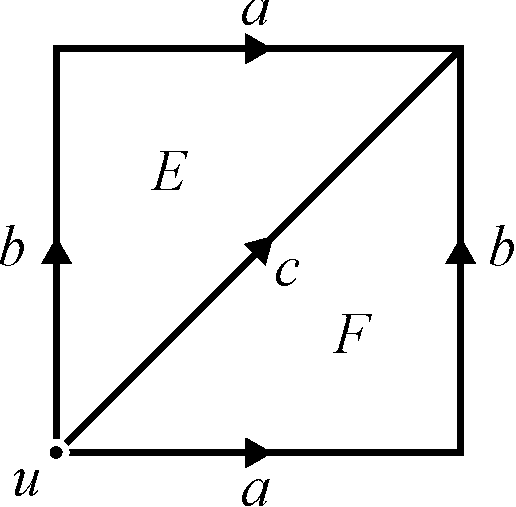
\includegraphics[width=0.4\columnwidth]{torus-delta.pdf}
	\caption[torus-delta]{$\Delta$-complex structure of a torus}
	\label{fig:torus-delta}
\end{figure}
The associated chain complex for taking simplicial homology is 
\begin{equation*}
	\begin{tikzcd}[row sep=tiny]
	\cdots & 0 & {E\Z \oplus F\Z} & {a\Z\oplus b\Z\oplus c\Z} & u\Z & 0 \\
	&&& {a,b,c} & 0 \\
	&& {E,F} & {a +b-c}
	\arrow["\partial_1", from=1-4, to=1-5]
	\arrow["\partial_2", from=1-3, to=1-4]
	\arrow[from=1-5, to=1-6]
	\arrow[from=1-2, to=1-3]
	\arrow[from=1-1, to=1-2]
	\arrow[maps to, from=3-3, to=3-4]
	\arrow[maps to, from=2-4, to=2-5]
\end{tikzcd}
\end{equation*}
Hence we get that
\begin{align*}
	H_0(\T^2) &\cong \Z,\\
	H_1(\T^2) &= \ker \partial_1 / \im \partial_2
	= a\Z \oplus b\Z \oplus c\Z / (a + b - c)\Z \cong \Z^2,\\
	H_2(\T^2) &= \ker \partial_2 = (E-F)\Z \cong \Z,
\end{align*}
and $H_n(\T^2) = 0$ for $n \geq 3$.
We deduce that the associated Betti numbers are
\begin{align*}
	b_0(\T^2) &= \rk(\Z) = 1,\\
	b_1(\T^2) &= \rk(\Z^2) = 2,\\
	b_2(\T^2) &= \rk(\Z) = 1,
\end{align*}
and $b_n(\T^2) = 0$ for $n \geq 3$.

\section{Weil Conjectures}
\label{sec:finite-fields}

For this section we fix a prime $p$ and $q$ a power of $p$.
We suppose throughout this section that $\chr(K) = p$.

In this section we will state the Weil conjectures and prove them in the
case of elliptic curve.

If $K$ is of characteristic $p$,
it contains a unique subfield of order $p^n$ for any $n \in \N$ (see
course \emph{Rings and Fields}), we will denote this subfield by $\F_{p^n}$.
We will be studying the set of
$\F_{q^n}$-rational points of a projective variety.

\begin{definition}
	Let $V/\F_q$ be a projective variety.
	The zeta function of $V/\F_q$ is defined as the power series
	\begin{equation*}
		Z(V/\F_q; T) = \exp\left(\sum_{n=1}^\infty (\#V(\F_{q^n}))
		\frac{T^n}{n}\right)
	\end{equation*}
\end{definition}

\begin{notation}
	When $V/\F_q$ is known from context, we write simply $Z(T)$
	instead of $Z(V/\F_q; T)$
\end{notation}

\begin{theorem}[Weil Conjectures]
	\label{thm:weil}
	Let $V/\F_q$ be a smooth projective variety of dimension $N$.
	\begin{enumerate}[label=(\alph*)]
		\item Rationality: $Z(T) \in \Q(T)$. More precisely, 
			there is a factorization
			\begin{equation*}
				Z(T) = \frac{P_1(T)\cdots P_{2n-1}(T)}
				{P_0(T)P_2(T) \cdots P_{2n}(T)},
			\end{equation*}
			where $P_0(T) = 1 - T, P_{2n}(T) = 1 - q^nT$ and for each
			$1 \leq i \leq 2n - 1$, $P_i(T)$ factors (over $\C$) as
			\begin{equation*}
				P_i(T) = \prod_j (1 - \alpha_{ij}T)
			\end{equation*}
		\item Functional Equation: The zeta function satisfies
			\begin{equation*}
				Z\left(\frac{1}{q^NT}\right) = \pm q^{N\frac{\epsilon}{2}}
				T^{\epsilon} Z(T),
			\end{equation*}
			for some integer $\epsilon$ (called the Euler characteristic of $V$)
		\item Riemann Hypothesis: $|\alpha_{ij}| = q^{i/2}$
			for all $1 \leq i \leq 2n - 1$ and all $j$.
		\item Betti Numbers: If $V/\F_q$ is a good reduction mod $p$ of a
			non-singular projective variety $W/K$, where $K$ is a number
			field embedded in the field of complex numbers, then the degree
			of $P_i$ is the $i$\textsuperscript{th} Betti number of the space
			of complex points of $W$. 
	\end{enumerate}
\end{theorem}

We won't define what a ``good reduction" means in general, but we can
look at the case of elliptic curves given by a Weierstrass equation.

If $K$ be a number field (seen as a subfield of its algebraic closure $\cl{K}$)
and $\O$ its ring of integers. Suppose $E$ is an elliptic curve given by a
Weierstrass equation defined over $K$, i.e. $E$ is of the form
\begin{equation*}
	E: y^2 = x^3 + ax + b
\end{equation*}
with $a, b \in K$. We have that $K = \Frac(\O)$ and so we can write
$a = a_1/a_2$ and $b = b_1/b_2$ for some $a_1, b_1 \in \O$, and
$a_2, b_2 \in \O\setminus\{0\}$.
We can decompose the ideal $(a_2b_2)$ into a product of prime ideals.
\begin{equation*}
	(a_2b_2) = \mf{p}_1\dots\mf{p}_s
\end{equation*}
Then choosing a prime ideal
$\mf{p}$ of $\O$ different from $\mf{p}_i$ for any $i$,
we get that $a_2, b_2 \notin \mf{p}$.
Hence we can see $E$ as being defined over $\O_\mf{p}$.
The maximal ideal $\mf{P}$ of $\O_\mf{p}$ is just the image of $\mf{p}$
under the localization. We deduce
\begin{equation*}
	\O_\mf{p}/\mf{P} \cong (\O/\mf{p})_\mf{p} = \O/\mf{p} \cong \F_q,
\end{equation*}
where $q$ is a power of $p$, where $(p) = \mf{p}\cap\Z$.

This gives us a new curve $C$ obtained by reducing $E$ modulo $\mf{P}$.

\begin{equation*}
	C: y^2 = x^3 + \bar{a}x + \bar{b},
\end{equation*}
defined over the residue field isomorphic to $\F_q$.
We say that $C$ is a \emph{good} reduction of $E$ modulo $p$
if it is also smooth. That is the case if and only if its discriminant
\begin{equation*}
	\Delta(C) = 4\bar{a}^3 + 27\bar{b}^2
\end{equation*}
is non-zero. But notice that the discriminant of $C$ is just the residue
of $\Delta(E) = 4a^3 + 27b^2$ modulo $\mf{P}$.
Hence the reduction of $E$ mod $p$ is ``good" if $\Delta(E) \not\in \mf{P}$.
We will show that (d) of \ref{thm:weil} holds for elliptic curves given
by Weierstrass equations in Section
\ref{sec:over-C}.

In the rest of this section, we will prove the Weil conjectures (save part (d))
for the case
of elliptic curves. For that, we will make use of the relation found in
\ref{prop:deg-tr-det}.
In the following proposition we get a formula for $\#E(\F_{q^n})$, which
we will be able to use for proving the Weil conjectures.

\begin{proposition}
	\label{prop:frob-char-poly}
	Let $E/\F_q$ be an elliptic curve, and
	\begin{equation*}
		\phi: E \to E, (x, y) \mapsto (x^q, y^q)
	\end{equation*}
	the $q$\ts{th}-power Frobenius endomorphism.
	Let $\alpha, \beta \in \C$ be the roots of the characteristic polynomial
	of $\phi_l$, that is
	\begin{equation*}
		\det(T - \phi_l) = T^2 - \tr(\phi_l)T + \det(\phi_l),
	\end{equation*}
	then $\alpha, \beta$ are complex conjugates satisfying
	$|\alpha| = |\beta| = \sqrt{q}$. Furthermore, for every $n \geq 1$, we
	have
	\begin{equation*}
		\#E(\F_{q^n}) = q^n + 1 - \alpha^n - \beta^n
	\end{equation*}
\end{proposition}

\begin{proof}
	We have by \ref{prop:frobenius-separable}
	and \ref{thm:preimage-card}
	that
	\begin{equation*}
		\#E(\F_q) = \deg(1 - \phi)
	\end{equation*}
	and from \ref{prop:deg-tr-det}, we have that
	\begin{equation*}
		\det(\phi_l) = \deg(\phi) = q;\\
	\end{equation*}
	For all $m/n \in \Q$, with $p \nmid m$,
	we have using \ref{prop:frobenius-separable} that
	\begin{equation*}
		\det\left(\frac{m}{n} - \phi_l\right)
		= \frac{\det(m - n\phi_l)}{n^2}
		= \frac{\deg(m - n\phi_l)}{n^2} \geq 0
	\end{equation*}
	Hence the polynomial $\det(T - \phi_l)$ is non-negative for $T \in \R$
	(by continuity). If $\alpha$, $\beta$ are the roots of $\det(T - \phi_l)$,
	it follows that $\alpha$, $\beta$ are complex conjugates (they can be
	equal). So $|\alpha| = |\beta|$ and since $\alpha\beta = \det(\phi_l) = q$,
	it follows that $|\alpha| = |\beta| = \sqrt{q}$.

	Now, for $n \geq 1$ the $(q^n)$\ts{th}-power Frobenius endomorphism
	$\phi^n$ satisfies
	\begin{equation*}
		\#E(\F_{q^n}) = \deg(1 - \phi^n) = \det(1 - \phi_l^n)
	\end{equation*}
	We have that
	\begin{equation*}
		\det(T - \phi_l^n) = (T - \alpha^n)(T - \beta^n)
	\end{equation*}
	since the eigenvalues of $\phi_l^n$ are the $n$\ts{th} powers
	of the eigenvalues of $\phi_l$. From 
	\ref{prop:deg-tr-det}, we have that
	\begin{equation*}
		\tr(\phi_l^n) = 1 + \deg(\phi^n) - \deg(1 - \phi^n)
		= 1 + q^n - \#E(\F_{q^n}).
	\end{equation*}
	and hence 
	\begin{equation*}
		\#E(\F_{q^n}) = 1 + q^n - \tr(\phi_l^m)
		= 1 + q^n - \alpha^n - \beta^n.
	\end{equation*}
\end{proof}

At last, we can state and prove the Weil conjectures for the case
of elliptic curves.

\begin{theorem}
	\label{thm:weil-elliptic}
	Let $E/\F_q$ be an elliptic curve. Then there exists an $a \in \Z$ such that
	\begin{equation*}
		Z(T) = \frac{1 - aT + qT^2}{(1-T)(1-qT)}.
	\end{equation*}
	Furthermore,
	\begin{equation*}
		Z\left(\frac{1}{qT}\right) = Z(T)
	\end{equation*}
	and
	\begin{equation*}
		1 - aT + qT^2 = (1 - \alpha T)(1 - \beta T)
	\end{equation*}
	with $|\alpha| = |\beta| = \sqrt{q}$
\end{theorem}

\begin{proof}
	Using the definition of $Z(E/\F_q; T)$, we get
	\begin{align*}
		\log Z(E/\F_q; T) &= \sum_{n=1}^\infty (\#E(\F_{q^n}))\frac{T^n}{n}\\
		&= \sum_{n=1}^\infty (q^n + 1 - \alpha^n - \beta^n)\frac{T^n}{n}
		\qquad \textrm{(\ref{prop:frob-char-poly})}\\
		&= -\log(1 - qT) - \log(1 - T) + \log(1 - \alpha T) + \log(1 - \beta T)
	\end{align*}
	and hence we get
	\begin{equation*}
		Z(E/\F_q; T) = \frac{(1 - \alpha T)(1 - \beta T)}{(1 - T)(1 - qT)},
	\end{equation*}
	which has the desired form.
	Indeed from (\ref{prop:frob-char-poly}), 
	$|\alpha| = |\beta| = \sqrt{q}$, and
	\begin{align*}
		a = \alpha + \beta = \tr(\phi_l) &= 1 + \deg(\phi) - \deg(1 - \phi)\\
		&= 1 + q - \#E(\F_q) \in \Z.
	\end{align*}
\end{proof}

Hence the Weil conjectures are verified for elliptic curves. Notice that
using the notation from theorem \ref{thm:weil},
$\deg P_0 = 1$, $\deg P_1 = 2$, $\deg P_2 = 1$, hence if $C/\F_q$ is a good
reduction of $E/K$, where $K$ is a number field embedded in
the field of complex numbers, we would expect
the Betti numbers of the space of complex points of $E$ 
to coincide with these values, and indeed, as we
will see in the following section, this is indeed the case.


\bibliographystyle{alpha}
\bibliography{references}

\end{document}
